\chapter{THEORETICAL FRAMEWORK}
\label{chp:frmwk}

The theoretical framework presented in this chapter provides a comprehensive exploration of key components and concepts essential for understanding the field of environmental sound recognition in embedded systems for autonomous vehicles. Starting with audio fundamentals, an in-depth analysis of microphones is presented, highlighting their role as capturing devices. This is followed by an exploration of machine learning and the utilization of neural networks, laying the foundation for the subsequent discussions on the classifiers and their potential application in environmental sound recognition algorithms. Finally, the chapter concludes by delving into the electronic control unit, elucidating its significance as a crucial element in the overall system architecture. 


\section{AUDIO FUNDAMENTALS}
\label{sec:frmwk_audio_fund}

This section provides a brief overview, definitions, and concepts of the fundamental aspects of audio laid down by \textcite{Mueller2016} and \textcite{Pelgrom2018}, setting the stage for a deeper exploration of environmental sound recognition.

\textbf{Frequency}, measured in hertz \gls{hz}, refers to the number of vibrations per second in a sound wave and plays a crucial role in determining the pitch of the sound. Higher frequencies are perceived as higher pitch, and vice versa. \textbf{Pitch}, in turn, encompasses the perception of the frequency of a sound and is logarithmic in nature, meaning the difference between two pitches of an octave is perceived as the same, regardless of their frequency values.

\textbf{Amplitude} measures the maximum displacement of a sound wave from its rest position. It is directly correlated with the loudness of a sound, as greater amplitude results in a louder sound. Additionally, an \textbf{octave} represents an interval between two frequencies where the higher frequency is double the lower frequency. This frequency relationship contributes to a logarithmic perception of pitch.

\textbf{Magnitude} is often associated with amplitude, signifying the strength or intensity of the sound wave. Meanwhile, \textbf{phase} refers to the position of a sound wave at a specific point in time, measured in degrees. It represents the progression of the wave cycle and is an essential aspect of understanding the characteristics of sound waves.

\textbf{Sound power} is the total acoustic energy produced by a sound source, measured in Watts.

\textbf{Sound intensity} (W/m\textsuperscript{2}) represents the power per unit area of a sound wave, quantifying the sound energy passing through a given area, and is measured in Watts per square meter. The concept of \textbf{intensity level}, expressed in decibels \gls{db}, serves as a logarithmic scale to measure sound intensity, allowing for the representation of a broad range of sound intensities.

\textbf{Loudness}, on the other hand, is the subjective perception of the intensity of a sound and is influenced by various factors such as sound pressure, frequency, and individual hearing characteristics. This subjective aspect ties closely to the objective measurement of sound intensity and intensity level.

Additionally, \textbf{timbre} plays a role in the overall perception of sound quality. Timbre refers to the perceived color or quality of sound that distinguishes one source from another. It is influenced by factors such as harmonic content, attack, and decay of the sound. Thus, the objective measurements of sound power and intensity connect to the subjective aspects of loudness and the distinctive quality of timbre in our perception of sound

The \textbf{sound envelope} represents the temporal evolution of a sound over time and is typically described using the \gls{adsr} model. It characterizes the initial attack, subsequent decay, sustained portion, and final release of a sound as depicted by the letters "A", "D", "S" and "R" in Figure \ref{fig:frmwk_audio_fund_adsr}.

\begin{figure}[htbp]
    \raggedright
        \caption{Waveform, amplitude envelope, and spectrogram representation for different instruments playing the same note C4 (261.6 Hz). (a) Piano. (b) Violin.}
        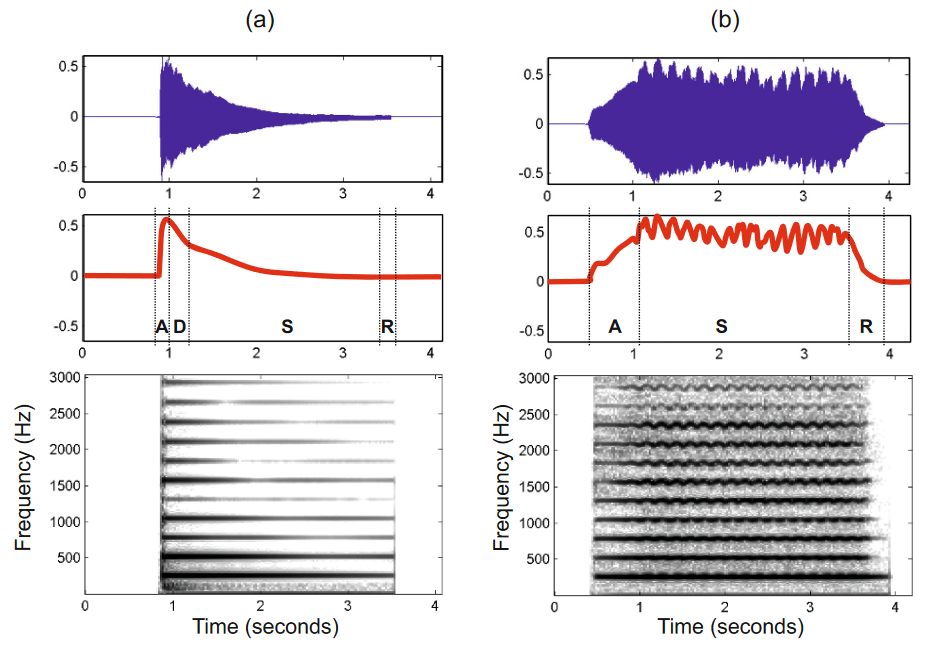
\includegraphics[width=0.9\textwidth]{resources/images/030-theoretical_framework/Framework_audio_fund_ADSR.png}
        \smallcaption{Source: \textcite{Mueller2016}, page 28}
        \label{fig:frmwk_audio_fund_adsr}
\end{figure}

The \textbf{threshold of audibility}, typically around 0 \gls{db} \gls{spl}, denotes the minimum sound level detectable by the human ear. In contrast, the threshold of pain, situated at approximately 120 \gls{db} \gls{spl}, represents the sound level at which sound becomes physically painful to the human ear. 

\textbf{\gls{adc}} involves two main processes: 
\begin{itemize}
    \item \textbf{Sampling} refers to capturing the value of an analog signal at discrete time intervals, while \textbf{sampling rate} determines the number of samples taken per second and is measured in \gls{hz}. In CD audio, the sampling rate is 44,100 \gls{hz}, meaning 44,100 samples are taken per second;
    \item \textbf{Quantization} focuses on the amplitude of the signal, essentially dividing the range of possible amplitudes into discrete levels. The number of quantization levels determines the resolution of the digital signal.
\end{itemize}

A \textbf{digital signal} is represented by a sequence of discrete values, typically binary digits (bits). It differs from the analog electrical signals created by a microphone, which have a continuous range of values.

The \textbf{resolution of a digital signal} is often specified in terms of the number of bits used for quantization, also known as the bit depth. Common bit depths include 16, 24, and 32 bits, with 16 bits being the standard resolution for audio CDs. For 1 minute (60 seconds) of audio at a sampling rate of 44,100 \gls{hz} and a bit depth of 16 bits, the required memory is 5.17 \gls{m}\gls{b}, calculated using the formula: 

\begin{equation}
    \label{eq:frmwk_audio_fund_audio_memory_calculation}
\text{Memory (MB)} = \frac{\text{Sampling rate} \times \text{Bit depth} \times \text{Duration}}{8 \times 1024}
\end{equation}

The higher the bit depth (or resolution) of a digital audio signal, the greater the dynamic range it can capture and reproduce. A higher bit depth allows for a more accurate representation of subtle changes in amplitude.

The digitization process in the \gls{adc} involves the quantization of the signal in time at a specific sampling rate and the quantization of its amplitude at a particular bit-depth. With the typical audio CD values above, these parameters efficiently capture the majority of perceptible information in the acoustic sound. The resultant digital representation of sound takes the form of a one-dimensional sequence of numbers, also known as a waveform, as illustrated in Figure \ref{fig:frmwk_audio_fund_digitization_process}.

\begin{figure}[htbp]
    \raggedright
        \caption{Two steps of a digitization process to transform an analog signal (solid curve) into a digital signal (stem plot). (a) Sampling. (b) Quantization.}
        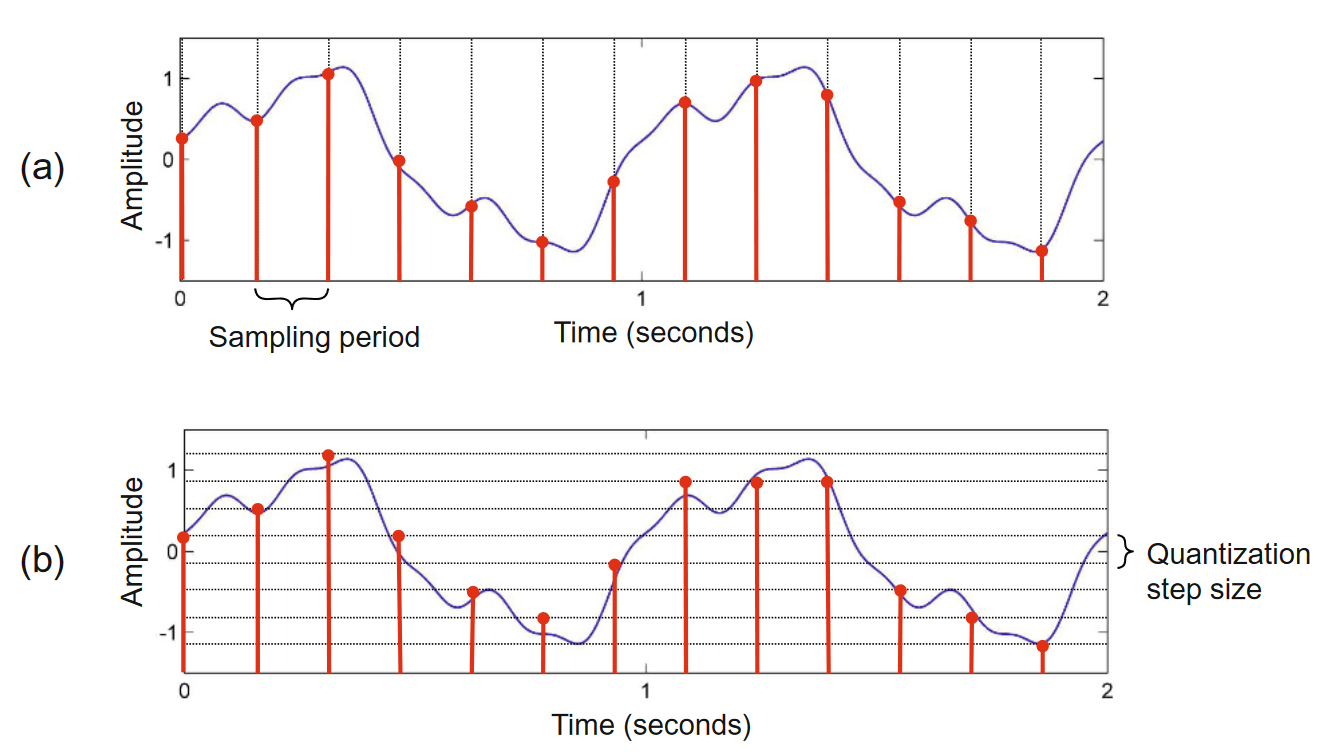
\includegraphics[width=1.0\textwidth]{resources/images/030-theoretical_framework/Framework_audio_fund_digitization_process.png}
        \smallcaption{Source: \textcite{Mueller2016}, page 61}
        \label{fig:frmwk_audio_fund_digitization_process}
\end{figure}

\textbf{Artifact} refers to an unintended and undesirable distortion or alteration of the audio signal that occurs during recording, transmission, processing, or playback. Artifacts can manifest as unwanted sounds, anomalies, or imperfections that degrade the quality of the audio signal.

According to the Nyquist-Shannon theorem, the \textbf{Nyquist frequency} is half the sampling rate. It represents the highest frequency that can be accurately represented in a digital signal without introducing distortion.

A \textbf{spectrogram} is a visual representation of the frequency content of a signal over time. It displays how the intensity of different frequencies in the signal changes over time, typically with frequency on the vertical axis, time on the horizontal axis, and color or brightness representing intensity


\subsection{Digital audio analysis}
\label{subsec:audio_fundamentals_digital_audio_analsys}

The conventional method for analyzing signals in the spectral domain relies on classical Fourier analysis, which is applied to the entire signal, shifting the information from the time domain to the frequency domain as shown in Figure \ref{fig:frmwk_digital_audio_fourier_transform}. However, the definition of the Fourier Transform faces challenges in audio signal analysis because real-world audio signals are time-varying. These signals are non-stationary, and their significance is inherently linked to this temporal variability. Therefore, there is a crucial need to develop techniques for analyzing sound that can capture the important time-varying aspects of audio signals, which are essential for feature extraction and other audio analysis tasks.

\begin{figure}[htbp]
    \raggedright
        \caption{Example of Fourier Transform applied to an audio signal illustrating the switch from the time domain to the frequency domain.}
        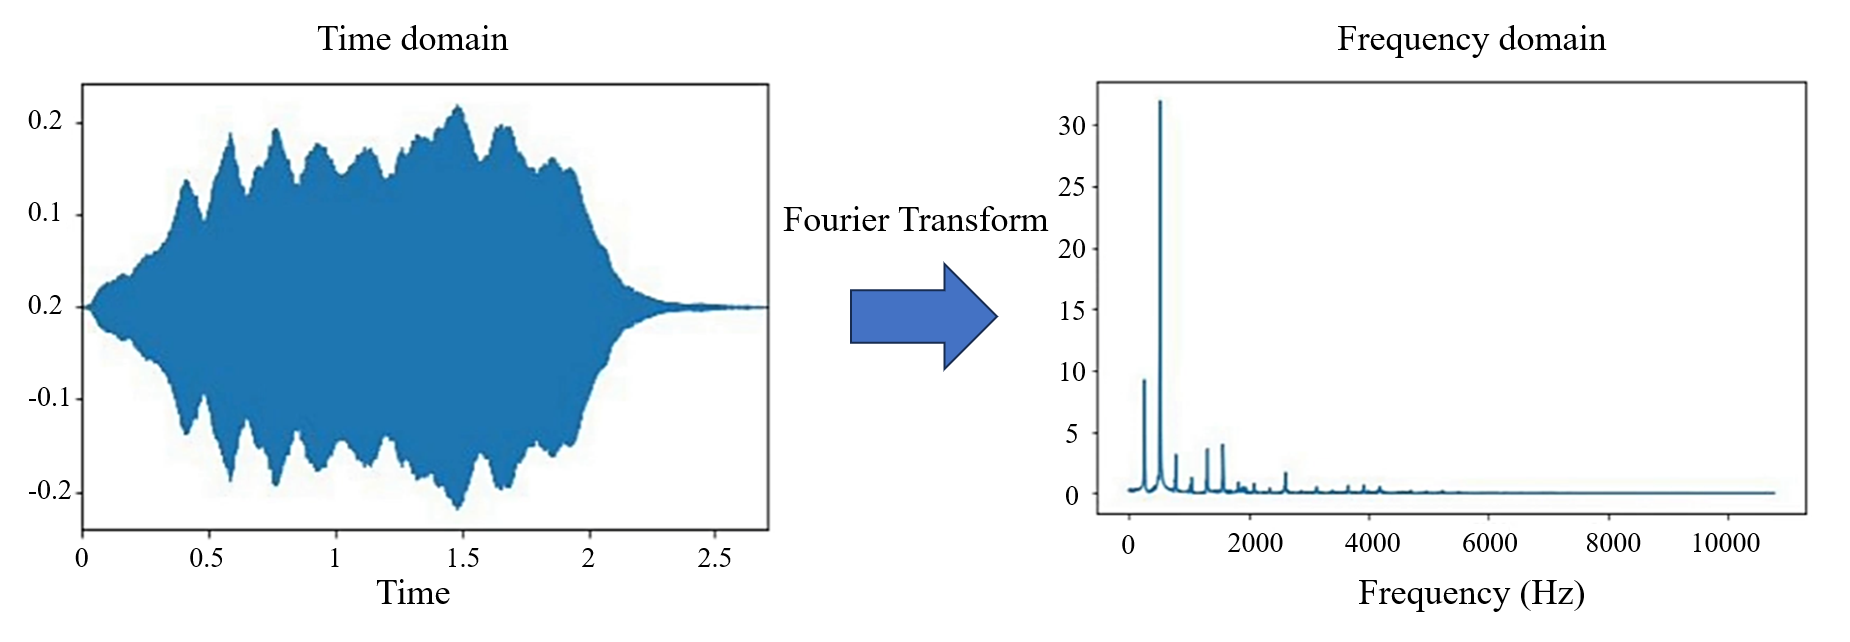
\includegraphics[width=1.0\textwidth]{resources/images/030-theoretical_framework/Framework_digital_audio_fourier_transform.png}
        \smallcaption{Source: Author}
        \label{fig:frmwk_digital_audio_fourier_transform}
\end{figure}

In order to overcome these challenges, the audio signal is initially divided into short segments called frames, and each frame is specifically chosen to be brief enough to be considered approximately stationary. This segmentation process is commonly referred to as \textbf{Framing}. The duration of each frame typically ranges from 10 to 50 \gls{mi}\gls{s}, assuming that within such a short timeframe, the audio signal undergoes minimal changes. Audio processing tasks, such as Fourier Transform and feature extraction, are performed on a frame-by-frame basis. To ensure a smoother transition and minimize abrupt changes and discontinuities that cause spectral leakage in the signal, frames are often multiplied by smoothing functions, such as the Hanning window function, prior to applying Fourier Transform operations, which renders this process the name \textbf{Windowing} \cite{Abreha2014}.

The technique of analyzing audio signals frame by frame is referred to as short-time signal analysis. In the existing literature \cite{Debnath2014}, there are various methods for short-time analysis, namely the \gls{stft}, Discrete Wavelet Transform (DWT), and Wigner-Ville Distribution (WVD). Among these, \gls{stft} stands out as the most commonly employed short-time analysis technique due to its computational simplicity.


\subsubsection{Short-Time Fourier Transform}
\label{subsubsec:audio_fundamentals_fourier_transform}

Joseph Fourier, born in 1768, made significant contributions to the field of mathematical physics, and he is particularly known for his work on heat transfer and the mathematical techniques he developed, including what is now known as the Fourier series and the Fourier Transform. His work on decomposing functions into sums of sinusoidal functions laid the foundation for the understanding of periodic functions and played a crucial role in various fields, including signal processing, communication theory, and quantum mechanics \cite{Debnath2014}.

The formula for the continuous complex Fourier Transform of a signal $f(t)$ is given by:

\begin{equation}
    \label{eq:frmwk_audio_fund_fft}
    \hat{f}(\omega)=\int_{-\infty}^{\infty} f(t) \cdot e^{-i \omega t} d t
\end{equation}

Where $\hat{f}(\omega)$ is the complex Fourier Transform of the signal at frequency $\omega$, the input signal is given by $f(t)$, the angular frequency by $\omega$, and the imaginary unit is $i$.

This formula involves integrating the product of the input signal and a complex exponential term over all time values $t$. The result is a complex-valued function of frequency $\omega$ that describes the frequency content of the input signal.

Given an analog signal $f : \mathbb{R} \rightarrow \mathbb{R}$ and a positive real number $T > 0$, the function $x : \mathbb{Z} \rightarrow \mathbb{R}$ is defined by $x(n):= f(n.T)$. Considering $x$ is defined only on a discrete set of time points, the value $x(n)$ is named \textbf{sample} taken at time $t = n.T$ of the original analog signal $f$ at the sampling period $T$, which is the inverse of the sampling rate.

In the context of discrete-time signals, the \gls{dft} is often used assuming, firstly, that most of the relevant information of $f$ is limited to a certain duration in time, resulting in a finite number of samples $x(0)$, $x(1)$, $\ldots$, $x(N-1)$ for some suitable number $N\in\mathbb{N} $, and secondly, one calculates the Fourier Transform for a limited set of frequencies. Analogous to discretizing the time axis, the frequency axis is commonly sampled with frequencies $\omega = k/M$ for some appropriate $M\in\mathbb{N} $ and $k \in [0: M-1]$. In practical applications, it is common to align the number $N$ of samples with the parameter $M$, determining the frequency resolution by setting $N = M$. It is essential to note that $N$ and $M$ refer to distinct aspects. Nevertheless, this alignment proves advantageous, ensuring not only the invertibility of the resulting transform but also yielding a computationally efficient algorithm \cite{Mueller2021}.

The formula for the \gls{dft} with integers $k \in[0:M-1]=[0:N-1]$ is given by:

\begin{equation}
    \label{eq:frmwk_audio_fund_dft}
    X(k) = \hat{x}(k / N)=\sum_{n=0}^{N-1} x(n) \cdot e^{-i 2 \pi n \frac{k}{N} }
\end{equation}

Where $\hat{x}(k/N)$ is the \gls{dft} of the signal at frequency index $k$, the input signal is $x(n)$, and $N$ is the length of the signal.

The \gls{dft} represents the frequency content of the signal at equally spaced frequency bins. In practice, the \gls{fft} algorithm is often used to efficiently compute the \gls{dft} by taking advantage of redundancies among sinusoids of various frequencies, allowing for the simultaneous computation of all Fourier coefficients through a recursive process. This recursion is especially effective when $N$ is a power of two, consequently, the \gls{fft} significantly decreases the total number of operations, reducing it from $O(N^2)$ to $O(N \log_2 N)$.

Instead of considering the entire domain of the signal, which hides "when" the frequencies occur, Dennis Gabor introduced in 1946, the \glsdisp{stft}{Short-Time Fourier Transform} (\gls{stft}) by focusing on specific sections of the signal or \textbf{frames}. This is achieved by multiplying the original signal with a \textbf{window function}, which defines the section being considered. By shifting the window function across time and performing a Fourier Transform on each windowed signal, frequency information at different time instances can be obtained. In other words, the \gls{stft} breaks the signal into frames, which overlap with each other to reduce artifacts at the boundary and to create more instances for analysis. 

Let a discrete signal $x$ be a function that maps integers to real numbers $\mathbb{Z} \rightarrow \mathbb{R}$. This signal is obtained by sampling at a regular rate $F_s$, given in \gls{hz}. Now let $w : [0:N - 1] \rightarrow \mathbb{R}$ be a sampled window function of length $N \in \mathbb{N}$. For example, considering a rectangular window, $w(n) = 1$ for $n \in [0:N - 1]$, outside this window, at time parameters not within $[0:N - 1]$, $w(n)$ will be assumed to be 0. The length parameter $N$ determines the duration of the sections (frames) considered in terms of $N/F_s$ seconds. Additionally, the parameter $H$ is introduced, a positive integer referred to as the \textbf{hop length}, which determines the number of samples by which the window is shifted across the signal \cite{Mueller2021}.

The formula for the discrete \gls{stft} $\mathcal{X}$ of the signal $x$ with $m \in \mathbb{Z}$ and $k \in [0:K]$ where $K = N/2$ (assuming that $N$ is even) is the frequency index associated with the Nyquist frequency is given by:

\begin{equation}
    \label{eq:frmwk_stft_discrete_stft}
    \mathcal{X}(m, k):=\sum_{n=0}^{N-1} x(n+m H) w(n) \cdot e^{-i 2 \pi n \frac{k}{N}}
\end{equation}

Where $\mathcal{X}(m, k)$ represents the $k^{th}$ Fourier coefficient for the $m^{th}$ time frame. For each time frame $m$, one gets a spectral vector of size $K+1$ given by its associated Fourier coefficients. The computational costs of each spectral vector amount to a \gls{dft} of size $N$, and as previously mentioned, it's more efficiently calculated using \gls{fft}. Figure \ref{fig:frmwk_stft_windowing} depicts this windowing process using a rectangular window function and a hop length of 50\%.

Assuming the total length (in samples) of an audio signal as $L$, the number of frames $m^{th}$ calculated using \gls{stft} is given by:

\begin{equation}
    \label{eq:frmwk_stft_frames}
    \text{Number of frames} = \left\lfloor \frac{L-N}{H} \right\rfloor + 1
\end{equation}

\begin{figure}[htbp]
    \raggedright
        \caption{Illustration of rectangular window function applied to an audio signal simulating the overlap of the frames.}
        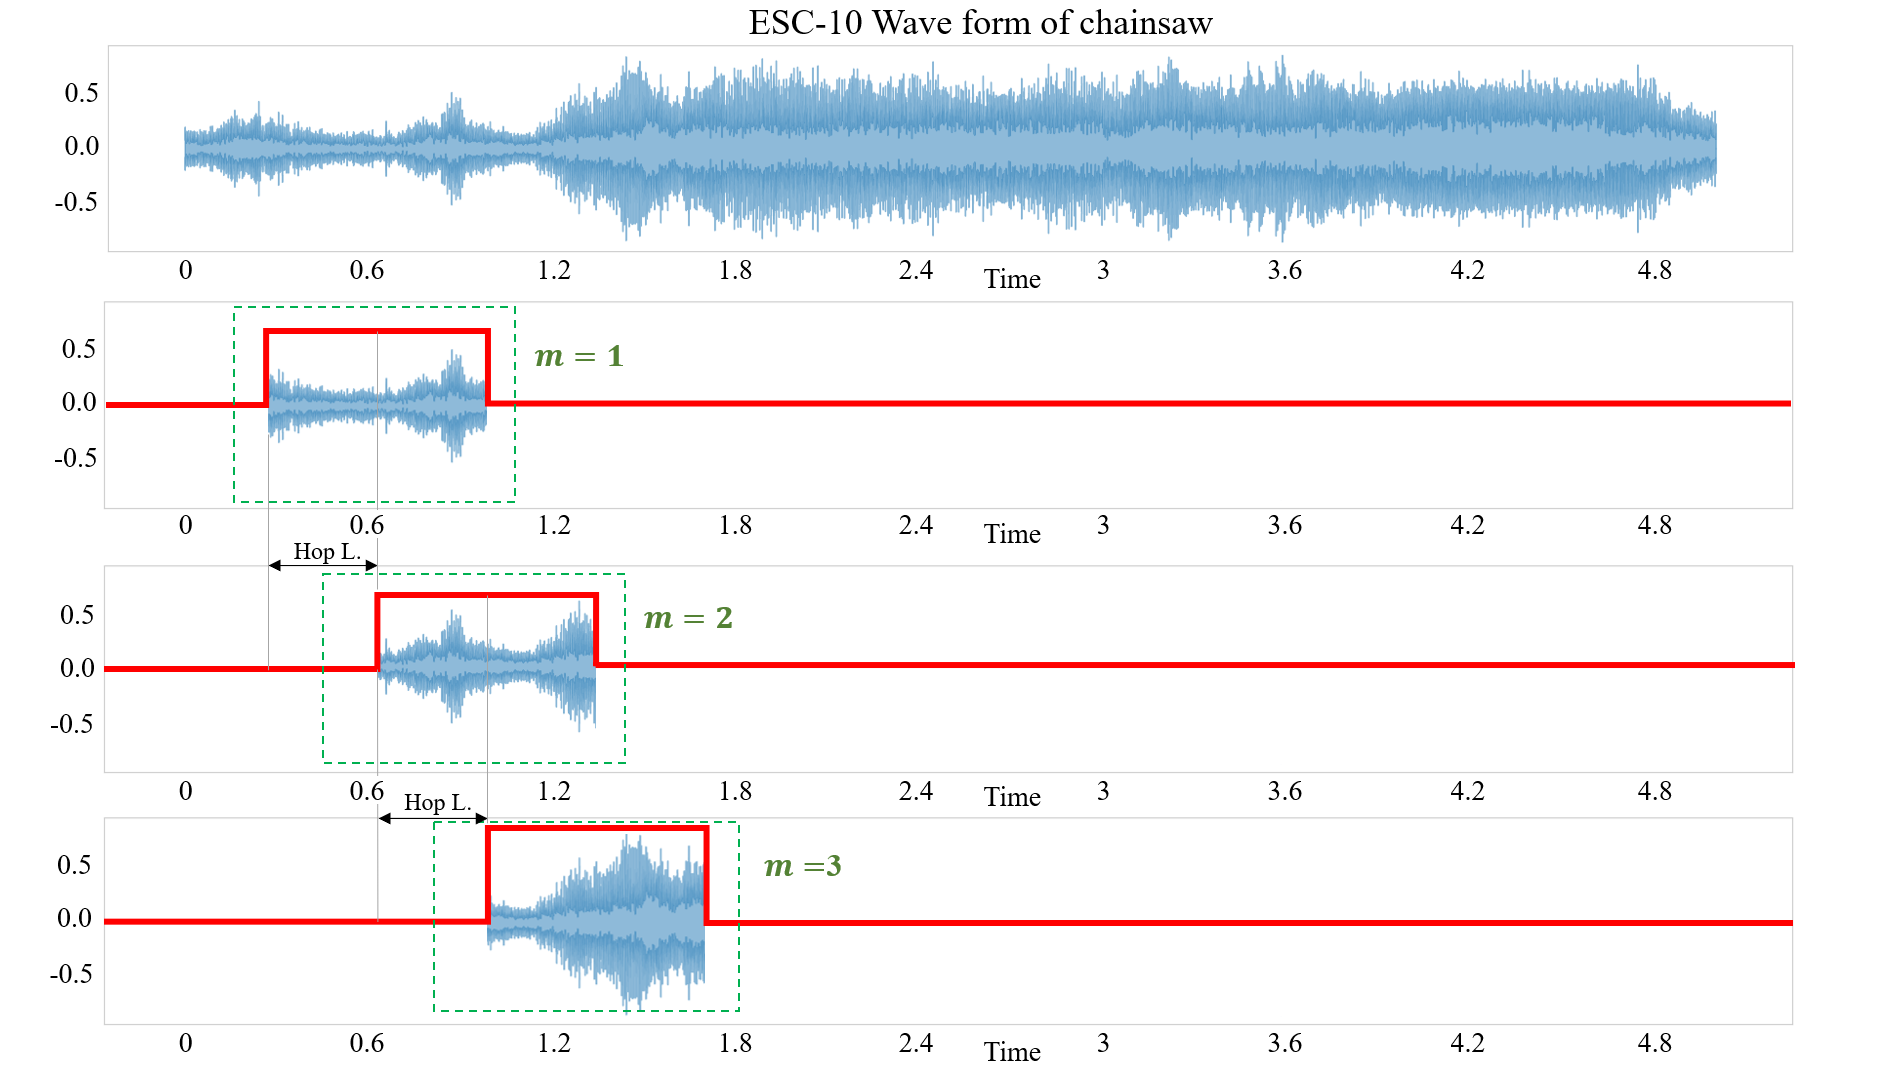
\includegraphics[width=1.0\textwidth]{resources/images/030-theoretical_framework/Framework_stft_windowing.png}
        \smallcaption{Source: Author}
        \label{fig:frmwk_stft_windowing}
\end{figure}


\subsubsection{Windows for the Short Time Fourier Transform}
\label{subsubsec:audio_fundamentals_windowing_techniques}

As already described, in audio analysis, techniques such as \gls{stft} are used to analyze sound by dividing the audio signal into smaller time segments called frames.  The length of each frame is typically chosen to balance the trade-off between time and frequency resolution, and overlapping frames are often used to improve the time resolution of the analysis. In the literature, a few types of framing have been utilized according to the end application, for example, \textcite{Preece2009} describe three types of framing to identify activities using body-mounted sensors: sliding windows, event-defined windows and activity-defined windows.

 Various window sizes have been utilized in earlier research, with some studies incorporating variable overlap between neighboring windows. Notably, the sliding window technique is straightforward and advantageous for real-time applications as it eliminates the need for pre-processing the audio signal. Its simplicity of implementation has made it the most commonly used approach for audio analysis and classification studies.

Considering the sliding window technique is the mainstream, the frames have to be synchronized or filtered using window functions. Several different windows are available named after their original developers in the 1950s, namely: Hamming window, Blackman window, Bartlett window (triangular), Hanning window (raised cosine window), and rectangular window \cite{Smith2013}, the last three illustrated in Figure \ref{fig:frmwk_windows_stft_example}. In \gls{stft}, a window function plays a crucial role in mitigating spectral leakage and managing trade-offs between time and frequency resolution by tapering the signal smoothly to zero at the edges thus minimizing abrupt transitions. The choice of window function influences the balance between main lobe width and side lobe levels, impacting the resolution of both time and frequency components in the resulting spectrogram. Named after Julius Von Hann, the \textbf{Hanning window} is one of the most used windows in signal processing according to \textcite{Mueller2021}.

\begin{figure}[htbp]
    \raggedright
        \caption{Windowed chirp signal and its magnitude Fourier Transform using different window functions. (a) Rectangular window. (b) Triangular window. (c) Hanning window.}
        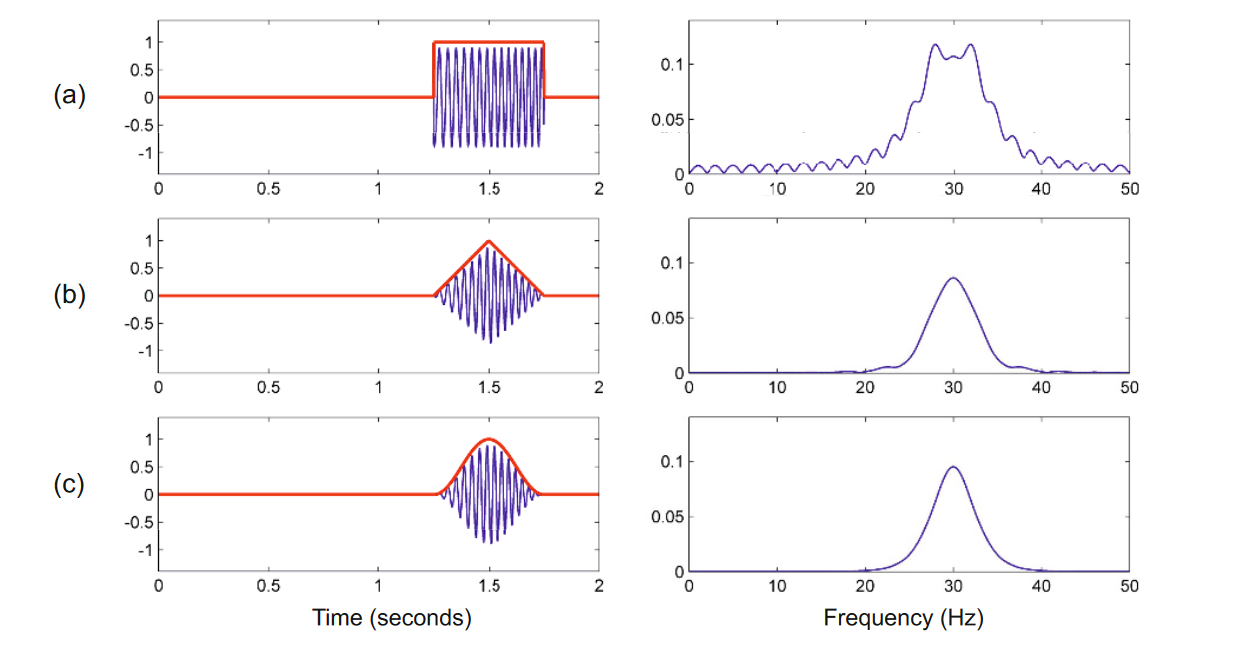
\includegraphics[width=1.0\textwidth]{resources/images/030-theoretical_framework/Framework_windows_stft_examples.png}
        \smallcaption{Source: \textcite{Mueller2021}, page 98}
        \label{fig:frmwk_windows_stft_example}
\end{figure}

Usually, the frame size and the Hanning window size have an equal number of samples, although, in some situations, one may choose different values for each one of them. Considering $w(n)$ is the value of the window at sample index $n$, and $N$ is the total number of samples in the window with $0 \leq n \leq N-1$, the Hanning window is mathematically defined according to \textcite{Smith2013} as:

\begin{equation}
    \label{eq:frmwk_windows_stft}
    w(n) = 0.5 - 0.5 \cos\left(\frac{2 \pi n}{N-1}\right)
\end{equation}


\subsubsection{Window function parameters}
\label{subsubsec:audio_fundamentals_window_function_parameters}

When performing a \gls{stft} using methods from specialized Python libraries such as openSMILE 3.0 \cite{Eyben2010} or \index{Librosa} Librosa \cite{McFee2015librosa_conf}, there are essentially three parameters that influence the result: window type, window size and overlapping size or hop length.

The choice of \textbf{window type} directly affects the result of the signal spectrogram. For instance, rectangular windows have a wide main lobe, providing high spectral resolution, but suffer from significant spectral leakage due to high side lobes, which causes a sudden interruption of the signal at its edges, possibly leading to incorrect estimations of frequency components. On the other hand, window types like Hamming and Hanning have narrow main lobes and lower side lobes, which reduce the signal's values towards zero at the edges of the window, preventing abrupt changes, resulting in a smoother spectrogram with reduced spectral leakage. The selection of an appropriate window type depends on the specific requirements of the application, such as the desired frequency resolution and the ability to distinguish between closely spaced spectral components \cite{Zoelzer2008}.

The \textbf{window size} parameter plays a vital role in determining the trade-off between time and frequency resolutions in the \gls{stft} analysis. The assumption is that within one frame, the signal is stationary, and the window size directly influences the temporal and frequency granularity of the resulting spectrogram. A smaller window size provides better temporal resolution, enabling the identification of rapid changes in the audio signal, however, it comes at the cost of reduced frequency resolution, making it challenging to distinguish between closely spaced frequency components accurately. Conversely, a larger window size improves frequency resolution but compromises temporal resolution. The choice of window size is typically application-dependent, where tasks requiring fine spectral details may necessitate smaller window sizes, while tasks focusing on temporal dynamics may benefit from larger window sizes. Notably, the terms "window size" and "frame size" refer to slightly different aspects but are closely related: the window size specifically refers to the length or duration (in samples) of the window function that is applied to segments of the audio signal during the \gls{stft} analysis while the frame size refers to the duration of the segments (in samples) into which the audio signal is divided before applying the window function \cite{Smith2013}. The output vector from a $N$-sample \gls{dft} of the audio signal sampled at $F_s$ results in $N/2 +1$ frequency bins, with each bin capturing the energy from a small range of frequencies in the original signal \cite{Abreha2014}, hence, the output vector of the \gls{stft} applied to $N$ samples results in an array of dimension: [frequency bins, number of frames] where the number of frames is given by equation \ref{eq:frmwk_stft_frames}. Most Python libraries implement their methods considering the window size and frame size to be identical, with the only option being to specify the frame size.

The process of overlapping frames guarantees that audio features present at a discontinuity are included in their entirety in the subsequent overlapped frame. The \textbf{overlapping size}, typically measured as a percentage, indicates the extent to which the previous frame is replicated in the following frame. Similar to selecting the window size, choosing the appropriate overlap size heavily depends on the specific objectives of the analysis or application. Generally, increasing the amount of overlap results in more analysis points and thus yields smoother results over time, potentially enhancing recognition accuracy in classification algorithms, however, this also leads to a proportional increase in computational cost. In Librosa \cite{McFee2015librosa_sw}, this parameter is named \textbf{hop length} and inputs an integer representing the number of samples overlapped.


\subsection{Audio features}
\label{subsec:audio_fundamentals_audio_features}

Essentially, there are two main types of audio features commonly used in the field of audio analysis: \textbf{physical features} and \textbf{perceptual features}. Physical features involve mathematical measurements derived directly from the sound wave, including the energy function, spectrum, cepstral coefficients, and fundamental frequency. On the other hand, perceptual features are subjective terms that relate to how sounds are perceived by humans, encompassing aspects such as loudness, brightness, pitch, timbre, and rhythm \cite{Zhang2010} and \cite{Alias2016}. Further on, physical features are further classified into \textbf{temporal features} and \textbf{spectral features}\footnote{For simplicity, frequency, image, and cepstral domains were all compiled in this classification}, which are based on the signal domain categorization. The selection of the following specific physical features for use in \gls{esr} applications was based on a comprehensive literature review presented in the related work chapter, but before that, a few definitions regarding feature categorization and requirements for feature selection were given.


\subsubsection{Requirements for selecting the audio features}
\label{subsubsec:audio_features_requirements_for_selecting_features}

Within the existing literature, numerous methods for extracting audio features are documented. The effectiveness of \gls{esr} heavily relies on the choice of audio feature extraction techniques utilized, and consequently, the careful selection of audio features becomes crucial in achieving optimal performance and accurate recognition. Even when constraining the application to \gls{esr}, the choice of audio features depends on the application’s type and purpose, particularly in resource-constrained devices like those used in the automotive industry, specifically for autonomous vehicles. The requirements for such implementation include multi-kernel support for end-to-end hybrid algorithms, real-time low-latency operation to quickly respond to each target event, and an optimized energy efficiency to reduce the overall vehicle power budget \cite{Yin2023}, nevertheless, these requirements can affect the recognition accuracy. Therefore, the selection of audio features should aim to develop a technique with low computational complexity, fast response time in the context of automotive applications, low energy consumption, and memory requirement, while still providing acceptable recognition accuracy. Given these requirements, the selection of audio features should include a small feature size to minimize computational cost, low computational complexity, high inter-class variability for improved discrimination between audio patterns, high intra-class similarity to decrease discrimination among similar classes, and low sensitivity to minor changes in the signal for robustness against noise and other sources of interference.


\subsubsection{Temporal features}
\label{subsubsec:audio_features_temporal}

Temporal features refer to characteristics or attributes of sound signals that evolve over time, making the temporal domain the native representation domain for audio signals. Extracted directly from the raw audio signal, temporal features do not require any preceding transformation, keeping the computational complexity low in comparison to spectral features. These features provide valuable information about the temporal dynamics of the audio signal. The temporal features included in this study are: \textbf{\gls{zcr}} and \textbf{\gls{rms}}.

\textbf{\gls{zcr}} is a low-level feature that captures the rate of transitions between positive and negative values within a signal, in other words,  the smoothness of a signal by counting the number of times the signal crosses the zero axis within a segment of that signal. It finds widespread application in fields such as speech recognition, music information retrieval, and percussive sound classification. Additionally, \gls{zcr} proves valuable in tasks like essential pitch detection for monophonic tonal signals and voice activity detection to ascertain the presence of human speech within audio segments \cite{Park2008}, it is sensitive to noise, though. 

\textbf{\gls{rms}} is another low-level feature that calculates the average energy of a frame and is an indicator of loudness that corresponds more closely to our hearing system’s sensitivity to the change in intensity of audio signals. It is less sensitive to outliers compared to amplitude envelopes and finds applications in audio segmentation and music genre classification. 


\subsubsection{Spectral features}
\label{subsubsec:spectral_fatures}

Spectral features refer to the characteristics or attributes extracted from the frequency domain representation of an audio signal aiming to capture specific spectral patterns or properties present in the signal. \textcite{Peeters2004} presents a large set of audio features, and most of them dwell in the frequency domain, so it's imperative to select the spectral features carefully. Each frequency or frequency bin provides information about its magnitude and phase, given that changes in phase have little impact on the perceived sound, there is no need to focus on features that analyze phase. Instead, the focus shifted to features that capture the basic properties of the sound's frequency distribution. Additionally, the spectral features utilized by \textcite{Lhoest2021}, \textcite{Silva2019}, and \textcite{Bountourakis2015}, provided a reliable direction. The spectral features included in this study are: \textbf{\gls{sc}}, \textbf{\gls{sb}}, \textbf{\gls{srp}}, \textbf{\gls{sct}}, \textbf{Tonnetz}, \textbf{Chroma feature}, \textbf{Mel spectrogram}, \textbf{\glsdisp{mfcc}{Mel-Frequency Cepstral Coefficients} (\gls{mfcc})}, and two feature manipulations namely: \textbf{Delta \gls{mfcc}} and \textbf{Delta-Delta \gls{mfcc}}.

\textbf{\glsdisp{sc}{Spectral Centroid} (\gls{sc})} can be interpreted as the "center of mass" or "center of gravity" of the spectrum of an audio signal. It is a measure of where the "center" of the spectral content of an audio signal lies in terms of frequency, and it is often used to describe the perceived "brightness" or "timbre" of a sound, and for that reason, sometimes is also addressed as a perceptual feature. It is a valuable feature for distinguishing between different types of sounds based on their spectral characteristics. %(Figure \ref{fig:frmwk_spectral_features_sc})
For example, sounds with higher spectral centroids tend to have a brighter or more treble-heavy quality, while those with lower centroids are generally more bass-heavy or darker in timbre \cite{Park2008}.

\textbf{\glsdisp{sb}{Spectral Bandwidth} (\gls{sb})} is another important feature that characterizes the width or spread of the frequency content in an audio signal's spectrum. It provides information about how concentrated or dispersed the spectral energy is across different frequency components. It also has a perceptual definition, commonly associated with the perceived "sharpness" or "clarity" of a sound. A higher spectral bandwidth indicates that the spectral energy is spread out over a broader range of frequencies, which can result in a sound perceived as being more complex or noisy. In contrast, a lower spectral bandwidth suggests that the energy is concentrated around a narrow band of frequencies, leading to a cleaner or purer sound \cite{Park2008}.

The \index{Librosa}Librosa \cite{McFee2015librosa_sw} method to extract \gls{sb} is based on \textcite{Klapuri2006}, but instead of calculating the second central moment of the spectrum, also known as spectral spread, using $p=2$, enables the computation of the $p-th$ root of the sum, where $p$ is left an input parameter ($p$ determines the "order" of the bandwidth calculation). 

\textbf{\glsdisp{srp}{Spectral Rolloff Point} (\gls{srp})} characterizes the frequency below which a specified percentage (often a threshold like 85\% or 95\%) of the total spectral energy lies, and it provides information about the lower boundary of the frequency range where most of the energy in an audio signal is concentrated. A higher spectral rolloff value indicates that the majority of the spectral energy is contained in lower frequencies, while a lower value suggests that energy extends into higher frequencies.

This feature is valuable for discerning voiced speech from unvoiced speech: the latter, including most of the environmental sounds, typically exhibits a significant concentration of energy in the higher frequency range of the spectrum, whereas voiced speech and music tend to have the majority of their energy concentrated in lower frequency bands. \cite{Giannakopoulos2014}. This study adopted the threshold of 85\%.

\textbf{\glsdisp{sct}{Spectral Contrast} (\gls{sct})} represents a way to describe the tonal characteristics or timbre of an audio signal. It is a feature that quantifies the difference in spectral energy between peaks and valleys in the frequency spectrum of an audio signal. Higher spectral contrast indicates greater variation in energy levels across frequency bands, which can lead to a perception of greater clarity and distinction between different parts of the sound spectrum. This can be relevant in tasks such as speech recognition, music analysis, and sound classification, where distinguishing between different frequency components is essential for understanding the content of the audio signal \cite{Jiang2002}.

Given a frequency domain divided into six Octave-scale sub-bands (0-200, 200-400, 400-800, 800-1,600, 1,600-3,200, and 3,200-8,000 \gls{hz}), \gls{sct} is computed by calculating the difference in energy between the maximum and minimum spectral values within each sub-band. The result is a multi-dimensional vector representing the contrast in energy between different frequency regions represented by the sub-bands.

\textbf{Chroma Feature} represents a way to describe the harmonic content or pitch class of an audio signal. It is a feature that characterizes the distribution of musical pitches (notes) in an audio signal, ignoring the octave or absolute frequency information. Chroma Features are typically computed using a chromagram, which is a representation of the 12 different pitch classes in Western music corresponding to the 12 semitones in an octave (e.g., C, C\#, D, D\#, E, F, F\#, G, G\#, A, A\#, B). One way to calculate Chroma Feature is, first, the audio signal is transformed into the frequency domain using techniques such as the \gls{dft}, then, for each short time frame of audio, the energy or magnitude of each of the 12 pitch classes is measured, resulting in a 12-dimensional vector that represents the presence or strength of each pitch class in that time frame \cite{Bartsch2005}.

Although similar in concept, Chroma Feature and \gls{sct} capture different aspects of the audio signal. Chroma Feature summarizes the distribution of energy in different pitch classes over time. \gls{sct}, on the other hand, focuses on capturing the difference in energy between peaks and valleys in the frequency spectrum. Chroma Features are computed by grouping frequency bins in the \gls{dft} spectrogram that correspond to the same pitch class and summing their magnitudes, while \gls{sct} is computed by dividing the spectrum into sub-bands, computing the mean energy within each sub-band, and then calculating the difference between the maximum and minimum energy across adjacent sub-bands.

\textbf{Tonnetz} represents a way to describe the tonal relationships or harmonic structure of an audio signal that characterizes the tonal distance between musical pitches (notes) in an audio signal using the concept of tonnetz, which is a two-dimensional representation of pitch space. To calculate Tonnetz features, first, the Chroma Features are extracted using the \gls{stft}, then the Chroma Features are converted to Tonnetz representation by using Euler's Tonnetz transformation. The result is a two-dimensional matrix or feature vector representing the tonal relationships between different pitch classes \cite{Harte2006}.

\index{Librosa}Librosa returns a vector  [6, $N$] where each row of Tonnetz values corresponds to the tonal centroid features for each frame $N$. The vector dimensions represent 0: Fifth x-axis, 1: Fifth y-axis, 2: Minor x-axis, 3: Minor y-axis, 4: Major x-axis and 5: Major y-axis.


The \textbf{Mel} Scale represents a significant advancement in our understanding of how humans perceive frequencies. Research has revealed that our perception of frequencies is not linear; rather, we exhibit greater sensitivity to differences in lower frequencies compared to higher ones. To illustrate, distinguishing between 500 and 1,000 \gls{hz} is relatively straightforward, while discerning a difference between 10,000 and 10,500 \gls{hz} proves considerably more challenging, despite the equal numerical interval between the two pairs. 

In 1937, Stevens, Volkmann, and Newmann introduced the concept of the Mel scale as a unit of pitch, designed to ensure that equal pitch intervals sounded equally spaced to the human ear. The name "Mel" originates from the musical term "melody," highlighting its connection to the frequency aspect of musical compositions and the measurement of pitch-related perceptual distances within melodies. To achieve this, a mathematical transformation is applied to frequencies, converting them into the \textbf{Mel scale}, thereby aligning auditory perception more closely with human sensitivity to frequency differences, in other words, the Mel scale is constructed such that sounds of equal distance from each other on the Mel scale, also “sound” to humans as they are equal in distance from one another having less resolution at high frequencies and a finer resolution at low frequencies \cite{Moore2013}. 

\textcite{Park2008} presents the original Mel scale curve in Figure \ref{fig:frmwk_spectral_features_mel_scale} (a) when $f_c$ is equal to $m$ at $f_c = 1$ \gls{k}\gls{hz} — the reference point between Mel frequency and frequency in Hertz, where 1 \gls{k}\gls{hz} is equal to 1,000 mels (the reference \gls{db} is 40 \gls{db} above the threshold of hearing). 

\begin{figure}[htbp]
    \raggedright
        \caption{Original Mel scale curve illustrating the intersection point where $f_c$ = 1\gls{k}\gls{hz} = 1,000 mels (a), and the common implementation utilized in Python and Matlab libraries with a linear response below $f_c$ = 1 \gls{k}\gls{hz} (b).}
        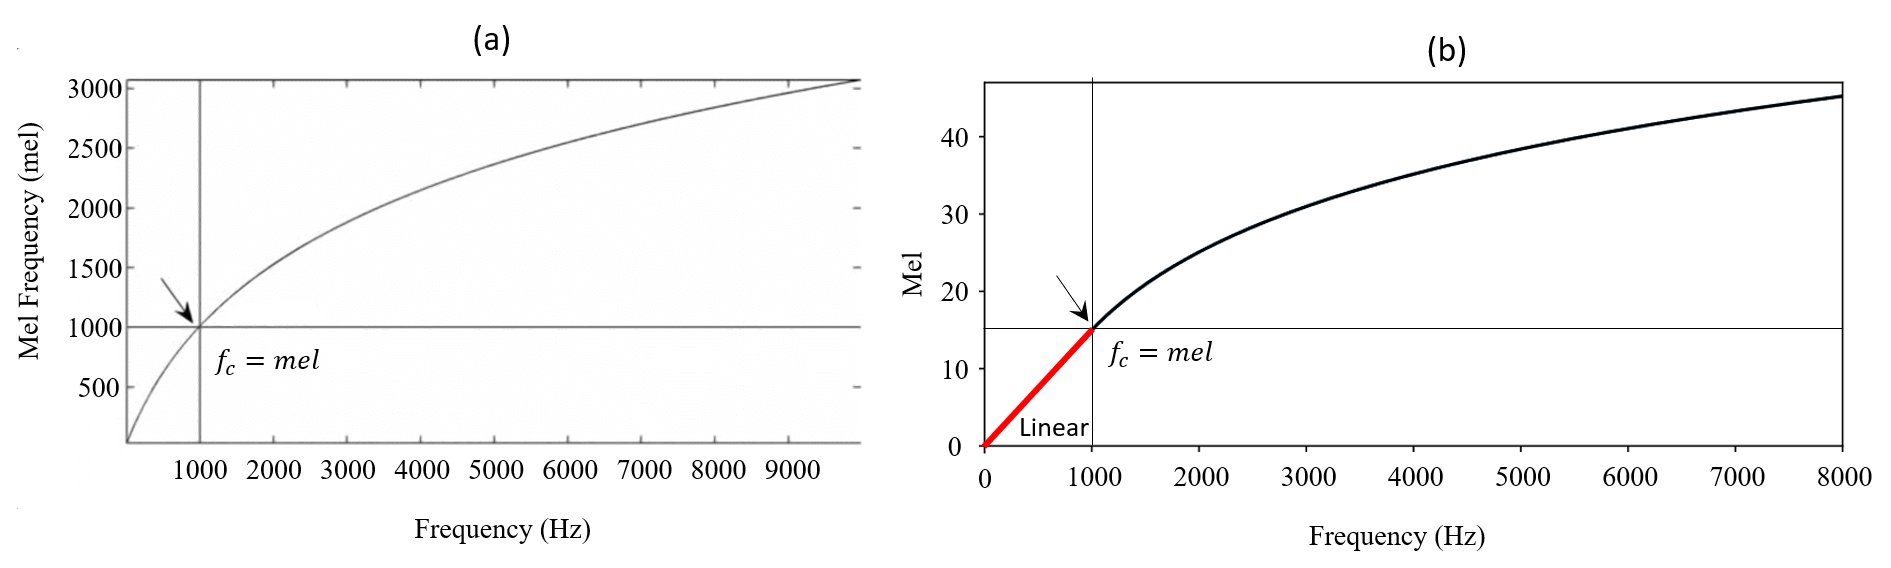
\includegraphics[width=1\textwidth]{resources/images/030-theoretical_framework/Framework_spectral_features_log-mel_scale.png}
        \smallcaption{Source: Author (a) "adapted from" \textcite{Park2008}, page 418, (b) "adapted from" \textcite{Rothmund2018}, page 68}
        \label{fig:frmwk_spectral_features_mel_scale}
\end{figure}

However, most current implementations in Matlab and Python, including \index{Librosa}Libosa, consider the auditory system’s frequency response as linear below $f_c = 1$ \gls{k}\gls{hz}, and upwards of $f_c$, the frequency resolution decreases incrementally, as depicted in Figure \ref{fig:frmwk_spectral_features_mel_scale} (b). 

\textbf{Mel spectrograms} are calculated by computing the \gls{stft} of the audio signal and mapping the result to the corresponding Mel scale using a mapping matrix. The matrix is based on $M$ triangular filters where each filter is scaled so that the area under each triangle is constant, as illustrated by Figure \ref{fig:frmwk_spectral_features_mel_filter_bank}. \index{Librosa}Librosa \cite{McFee2015librosa_sw} returns a vector [$M, N$] where each row of Mel band $m$ has the mel-spectrogram magnitude of the frequency bins $k$.

\begin{figure}[htbp]
    \raggedright
        \caption{Mel-weighting filter bank consisting of 8 triangular filters combing linearly spaced frequency bins between 0 and 8 \gls{k}\gls{hz} into 8 Mel bands from 100 \gls{hz} to 6 \gls{k}\gls{hz}}
        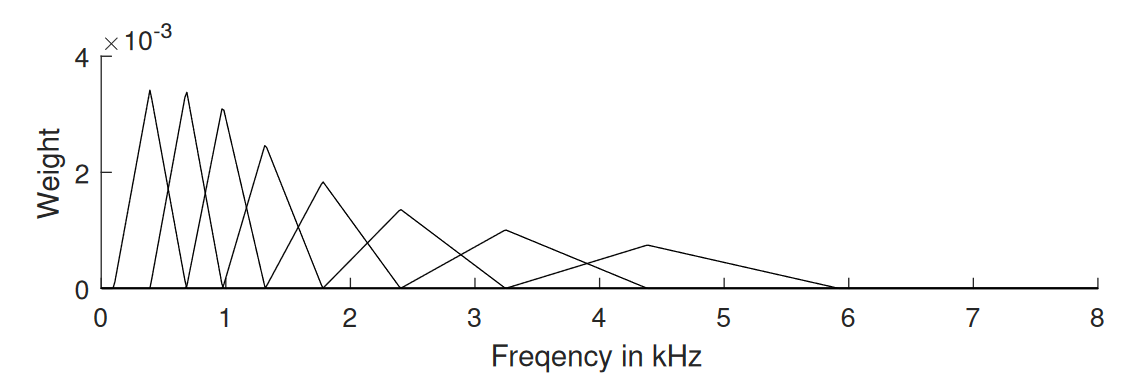
\includegraphics[width=.75\textwidth]{resources/images/030-theoretical_framework/Framework_spectral_features_log-mel_filter_bank.png}
        \smallcaption{Source: \textcite{Rothmund2018}, page 69}
        \label{fig:frmwk_spectral_features_mel_filter_bank}
\end{figure}

The concept of \textbf{\glsdisp{mfcc}{Mel-Frequency Cepstral Coefficients} (\gls{mfcc})} was originally introduced in the 1980s for speech recognition tasks \cite{DavisMermelstein1980}, aimed to address the limitations of simple spectral analysis techniques, which were found to be inadequate for representing the characteristics of human speech. Cepstrum and quefrency were coined by swapping the initial syllables of spectrum and frequency. According to \textcite{Oppenheim2004}, this consonant exchange illustrates the cross-disciplinary approach, where techniques typically used in the time domain are applied to frequency analysis and vice versa. Although very popular in the field of speech recognition, it also found space in the field of audio classification, being rated as the most utilized feature extraction technique in the systematic review of data augmentation and deep learning methods in sound classification \cite{Alli2022}.

The computation of \gls{mfcc} involves several steps according to \textcite{Klapuri2006}:

\begin{itemize}
    \item A pre-emphasis filter is applied to flatten the spectrum;
    \item The audio signal is framed, windowed, and transformed using the \gls{dft};
    \item A Mel-scale filter bank is applied in the frequency domain, as previously explained;
    \item The power within each sub-band is computed by squaring and summing frequency bin magnitudes within bands;
    \item The dynamic range of the spectrum is compressed by taking a logarithm of the band-wise power values;
    \item Finally, cepstral coefficients are computed by applying, to the log filter bank powers, the \gls{dct}\footnote{The Discrete Cosine Transform is similar to the \gls{dft} but only uses the cosine function to represent the signal.} which decorrelates the coefficients as:
\end{itemize}

The dimensionality of the representation can be reduced by retaining only approximately 13 lowest-order \gls{dct}, which usually carry the relevant timbral information. Succinctly, the first \gls{dct} coefficient serves to denote the average power or energy in the spectrum, the second coefficient offers an approximation of the spectrum's broad shape and maintains a relation to the spectral centroid, whereas, for the higher-order coefficients, they capture finer spectral details such as pitch. Typically, in practice, a subset ranging from the first 8 to 13 \gls{mfcc} coefficients adequately represents the spectrum's shape, with the higher-order coefficients being disregarded due to their redundancy in providing additional information \cite{Abreha2014}. Librosa returns a vector [$\sum i, N$] where each row $i$ has the \gls{mfcc} coefficients of the frequency bins $k$.

\gls{mfcc} has one significant limitation: is its sensitivity to noise and channel variations. If the audio signal is corrupted with noise or transmitted through a poor-quality channel, the extracted \gls{mfcc} coefficients may not accurately represent the underlying sound information. Another limitation is the lack of temporal information in the \gls{mfcc} representation. Since the computation of \gls{mfcc} is frame-based, it does not capture the dynamics and temporal variations of the speech signal. To alleviate this limitation, dynamic features such as delta and acceleration coefficients are commonly computed by taking the derivatives of \gls{mfcc} \cite{Gold2011}. To illustrate this concept, Figure \ref{fig:frmwk_spectral_features_mfcc} compares the spectrograms of the \gls{mfcc} (first row), $\triangle$\gls{mfcc} (second row), and $\triangle\triangle$\gls{mfcc} (third row) set to 13 coefficients for five samples from the ESC-10 dataset, 

\begin{figure}[htbp]
    \raggedright
        \caption{Example of \gls{mfcc}, $\triangle$\gls{mfcc}, and $\triangle\triangle$\gls{mfcc} plots applied to random samples of the dataset ESC-10.}
        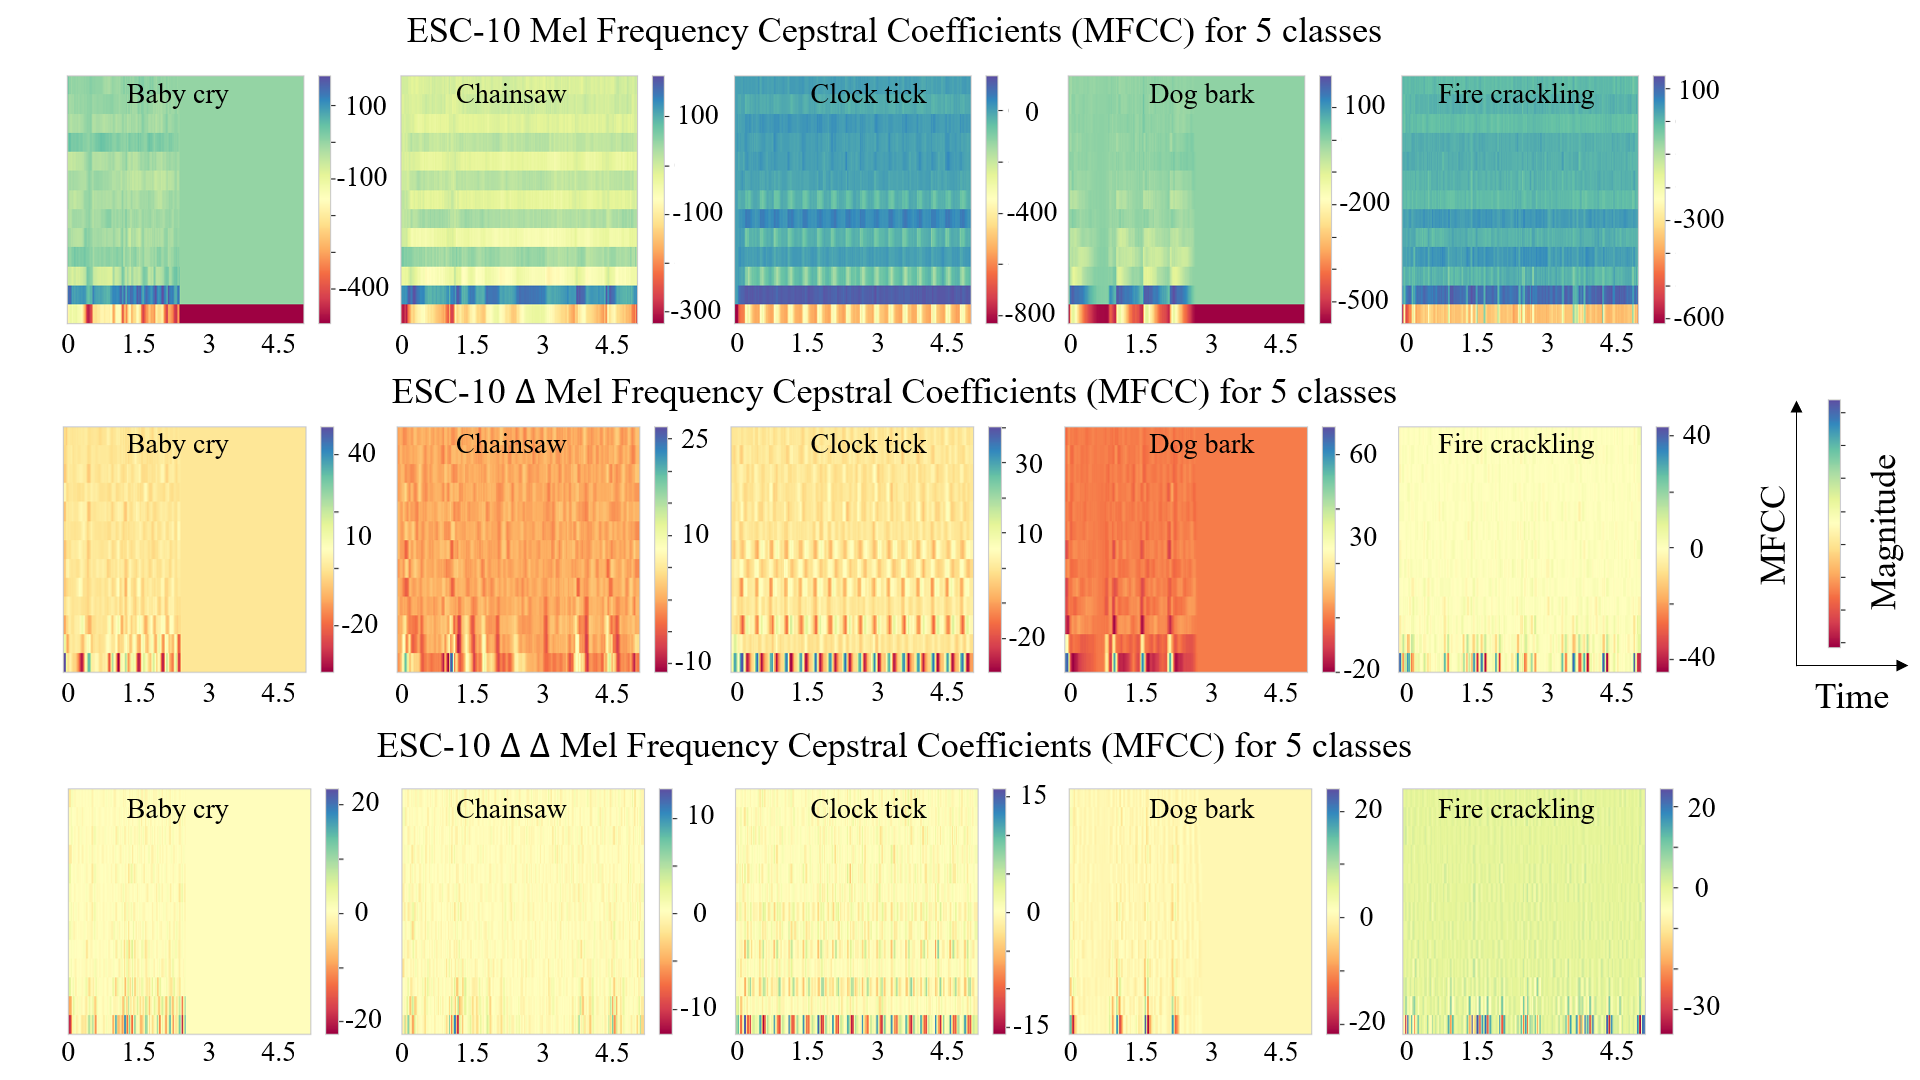
\includegraphics[width=1.0\textwidth]{resources/images/030-theoretical_framework/Framework_spectral_features_mfcc.png}
        \smallcaption{Source: Author}
        \label{fig:frmwk_spectral_features_mfcc}
\end{figure}

\textbf{Delta \gls{mfcc}} and \textbf{Delta-Delta \gls{mfcc}}, also known as \textbf{$\triangle$\gls{mfcc}} and \textbf{$\triangle\triangle$\gls{mfcc}}, are the first and second-order derivatives of the \gls{mfcc} along the time axis. The first captures information about the velocity or speed of changes in the audio features, and the latter captures the rate of change of the $\triangle$\gls{mfcc} coefficients, capturing the curvature or acceleration of the spectral features. Both $\triangle$\gls{mfcc} and $\triangle\triangle$\gls{mfcc} are often concatenated with the original \gls{mfcc} coefficients to form a feature vector that incorporates temporal dynamics \cite{Bountourakis2019} and \cite{Tang2018}. 


\subsection{Conclusion}
\label{subsec:audio_fundamentals_conclusion}

Based on the detailed exploration of audio feature extraction techniques in the context of \gls{esr}, it became evident that selecting appropriate audio features plays a critical role in achieving optimal performance and accurate recognition. The unique requirements of \gls{esr} for autonomous vehicles, such as multi-kernel support, real-time operation, energy efficiency, and memory optimization, present challenges that must be carefully considered when choosing audio features. The ideal audio features for such applications should exhibit low computational complexity, fast response time, minimal energy consumption, and memory usage while maintaining acceptable recognition accuracy, all of which can be achieved with the selected features using \gls{stft}. Additionally, the chosen audio features should possess a small feature size to reduce computational costs, and therefore, \gls{mfcc}, \gls{sct}, Chroma, and Tonnetz must be carefully assessed in terms of their influence on the classification metrics.


\section{MICROPHONES}
\label{sec:frmwk_microphones}

This section introduces relevant definitions, concepts, and characteristics related to microphones, hearing capabilities, and their applications in the automotive industry. It will also evaluate the null hypothesis: a regular passenger car microphone has auditory sensitivity higher than or equivalent to human ears.


\subsection{Definitions}
\label{subsec:microphones_definitions}

In psychoacoustics, \textbf{sensitivity} is the ability of the human ear to detect and comprehend sounds at various frequencies and intensities, measuring how well an individual can perceive and differentiate sounds at different levels of volume or loudness \cite{Moore2013}.

In a microphone, \textbf{sensitivity} represents the ability to convert sound waves into an electrical signal. It measures how well a microphone can collect and detect sound, especially low-level or quiet noises, which means a microphone's sensitivity dictates how responsive it is to sound pressure levels and influences its ability to capture quiet or distant sounds accurately. Sensitivity is often evaluated as the \gls{spl} necessary to achieve a specific output level from the microphone and is usually represented in \gls{db}. The higher the sensitivity rating in \gls{db}, the more sensitive the microphone is to sound \cite{Rayburn2004}.

\textbf{\gls{fr}} refers to how well the human ear can perceive sound at different frequencies in psychoacoustics. It measures the sensitivity of the human ear to sound at various frequencies, and it plays a vital role in determining how humans perceive and interpret different sounds. The human ear's frequency sensitivity does not remain constant across all frequencies; rather, some frequencies are more responsive to the ear than others. A \gls{fr} curve, which illustrates how well the ear responds to different frequencies, can be used to measure this sensitivity, and it typically depicts the amount of sound pressure required for a listener to perceive a sound at a specific frequency, measured in \gls{db} and plotted with frequency (in \gls{db}) on the horizontal axis and \gls{spl} on the vertical axis \cite{Moore2013}.

In a comparable manner, \textbf{\gls{fr}} in a microphone refers to how it responds to different frequencies across the audible spectrum, in other words, it describes the microphone's ability to capture and reproduce sound accurately at various frequencies \cite{Rayburn2004}.

A microphone's frequency response is often displayed as a graph or numerical specification that demonstrates how the sensitivity of the microphone fluctuates across the frequency range. According to \textcite{Rayburn2004} and illustrated in Figure \ref{fig:frmwk_microphone_frequency_response}, the microphone's frequency response shows which frequencies are more responsive to the microphone and how it attenuates or highlights specific frequency ranges.

\begin{figure}[htbp]
    \raggedright
        \caption{Amplitude response versus frequency with upper and lower limits for a capacitor vocal microphone; the effect of lower frequency cut is also shown.}
        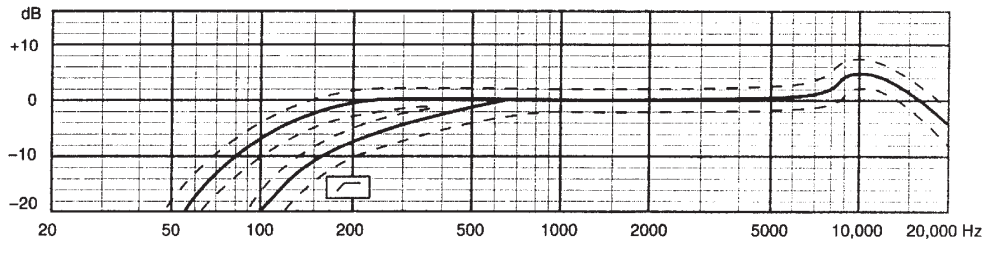
\includegraphics[width=1\textwidth]{resources/images/030-theoretical_framework/Framework_microphone_frequency_response.png}
        \smallcaption{Source: \textcite{Rayburn2004}, page 106}
        \label{fig:frmwk_microphone_frequency_response}
\end{figure}

\subsection{Human hearing capabilities}
\label{subsec:microphones_Human_hearing_capabilities}

The range of sound intensity (pressure) and frequency to which the ear responds is truly astonishing, as presented in Figure \ref{fig:frmwk_microphone_human_hearing} below. The intensity ratio between painful noises and the weakest sounds humans can hear is greater than $10^{12}$, and the frequency ratio between the highest and lowest frequencies humans can listen to is roughly 1,000 times greater (20 \gls{hz} and as high as 20,000 \gls{hz}), or more than nine octaves - each octave represents a frequency doubling \cite{Rossing2013}. The auditory system's selectivity is another noteworthy feature, and also according to \textcite{Rossing2013}, a listener can discern the sound of a solo instrument among the blended sounds of a symphony orchestra, it is possible to distinguish a single speaker in a crowded room, a mother's conditioned ear can respond to an infant's cry even while she is sleeping and one may even teach himself to sleep through city traffic noise but wake up at the sound of an alarm clock or odd noise.

In general, the frequency response of the human ear is highest in the range of 2-4 \gls{k}\gls{hz} and gradually decreases at higher and lower frequencies, as illustrated in Figure \ref{fig:frmwk_microphone_human_hearing} by the curves of threshold of pain and threshold of audibility \cite{Moore2013}.

\begin{figure}[htbp]
    \raggedright
        \caption{Range of frequencies and intensities to which the auditory system (ear) responds.}
        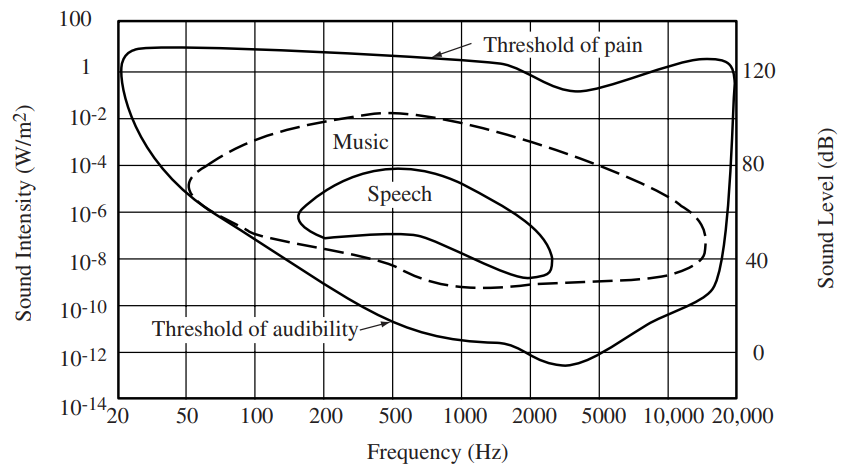
\includegraphics[width=1\textwidth]{resources/images/030-theoretical_framework/Framework_microphone_human_hearing.png}
        \smallcaption{Source: \textcite{Rossing2013}, page 80}
        \label{fig:frmwk_microphone_human_hearing}
\end{figure}


\subsection{Automotive vehicle microphones}
\label{subsec:microphones_automotive_vehicle}

There is a relatively small body of literature that is directly related to the types of microphones commonly used in regular passenger cars. In general, they are used in automotive vehicles for a variety of purposes, including hands-free calling, voice-activated controls, and in-car entertainment systems \cite{Newcomb2008}. The ones listed below are the microphone types commonly used in regular passenger cars according to \textcite{Rumreich2005}:

\begin{itemize}
    \item Built-in microphones: many modern vehicles come with built-in microphones integrated into the cabin's dashboard or ceiling. These microphones are often used for hands-free calling and voice-activated controls and are typically designed to pick up sound from within the cabin;
    \item Headset microphones: some vehicles come with headsets that have built-in microphones, which can be worn by the driver or passengers to communicate with other passengers or with the vehicle's audio system. These microphones are typically small and lightweight and are designed to be comfortable to wear for extended periods;
    \item External microphones: in some cases, external microphones may be used in automotive vehicles to pick up sound from outside the cabin, such as using a hands-free calling system while driving with the windows down. These microphones are typically designed to be weather-resistant and durable and may be mounted on the vehicle's exterior;
    \item Bluetooth microphones: many modern vehicles are equipped with Bluetooth technology, allowing users to wirelessly connect their smartphones or other devices to the vehicle’s audio system. Bluetooth microphones are commonly used for hands-free calling and voice-activated controls and are designed to be small and unobtrusive.
\end{itemize}

Overall, the type of microphone used in a product will depend on the specific application and the design of the product's audio system. There seems to be a trend in the automotive industry to design audio systems using built-in and Bluetooth microphones, however, in some cases, external microphones may be necessary to achieve the desired level of sound quality and clarity \cite{Rayburn2004}.

Built-in microphones are commonly used in the automotive industry as hardware modules equipped with interfacing circuitry and connectors. To detect acoustic signals, these microphones use either a single microphone element for voice sensing in hands-free calling or multiple elements for signal sensing, including \gls{anc} in the case of beam-forming applications. In particular, \gls{ecm} and \gls{mems} microphone elements are widely utilized in automotive microphone modules and are essential in controlling the acoustic performance of the module \cite{Aubauer2001}. The advancements in microphone elements' signal-to-noise ratio and acoustic overload point specifications do not necessarily improve end-users' experience or \gls{si} in an automotive environment. Even when a simulation model is developed to investigate the impact of microphone element sensitivity and phase mismatches on beam-forming performance, the results show significant dependency on the chosen array processing algorithm \cite{Du2019}. 

\textcite{Du2022} investigated the \gls{si} of hands-free microphones used in vehicle audio systems, measured by a score (\gls{si} score), which is considered an important performance metric and cannot be directly obtained from the microphone datasheet. They categorized the three most common microphone types in the automotive industry:

\begin{itemize}
    \item Omnidirectional with a flat \gls{fr} shape in the entire speech band (e.g., 20-14.000 \gls{hz});
    \item Omnidirectional with a rising \gls{fr} shape and a -3 \gls{db} cut-off frequency between 100 and 500 \gls{hz};
    \item Unidirectional (e.g., Cardioid) microphone.   
\end{itemize}

Based on their experiments, they concluded that at low background noise levels, there are no noticeable differences in intelligibility among the three microphones. However, in the presence of medium to high-level and non-wind-induced noises, the unidirectional or omnidirectional microphone with a rising frequency response shows certain advantages over the omnidirectional microphone with a flat \gls{fr}. On the other hand, in the presence of wind turbulence-induced noises, which are typically at high levels, the unidirectional microphone exhibits the greatest performance degradation.


\subsection{Conclusion}
\label{subsec:microphones_conclusion}

Based on the body of literature investigated, it can be inferred that the maximum attainable sensitivity level of the microphones typically employed in the automotive industry is conventionally constrained by the caliber of the microphone's transducer and the electronic signal processing circuitry utilized to analyze the acoustic beam forming. Despite exhibiting noteworthy electroacoustic characteristics, they demonstrate limited potential in attaining the discernment and precision achievable by the human auditory system, and therefore, the null hypothesis is rejected. Nevertheless, it is imperative to note that these microphone types do exhibit sufficient attributes capable of detecting a substantial range of acoustic events. This inference imparts significant technological insights regarding using automotive microphones in environmental sound recognition.


\section{MACHINE LEARNING}
\label{sec:frmwk_machine_learning}

Machine learning plays a crucial role in enabling autonomous systems to acquire knowledge, make informed decisions, and adapt to dynamic environments. Within the context of \gls{esr}, the current literature predominantly focuses on supervised learning for classification tasks due to its effectiveness and practical applicability. However, semi-supervised and reinforcement learning approaches are also present, primarily for audio tagging tasks. 


\subsection{Classification}
\label{subsec:machine_learning_classification}

In a broader definition given by \textcite{Russel2010}, any component of an agent can be improved by learning from data, essentially depending on four major factors: which \textit{component} is to be improved, what \textit{prior knowledge} the agent already has, what \textit{representation} is used for the data and the component, and what \textit{feedback} is available to learn from.

There are three types of feedback that determine the three main types of learning, with one variation that could be classified as the fourth \cite{Russel2010}:

\textbf{Unsupervised learning} is characterized by the absence of explicit feedback or labeled examples during the learning process. Instead, the agent focuses on recognizing patterns and structures within the input data. By detecting and clustering potentially meaningful groups or clusters of input examples, the agent can uncover valuable insights without external guidance or supervision. An example of unsupervised learning in the domain of environmental sound recognition could involve an autonomous taxi agent gradually developing the concept of "good traffic days" and "bad traffic days" based solely on the audio patterns it observes, without being explicitly provided with labeled examples by a teacher.

\textbf{Reinforcement learning} revolves around using a series of reinforcements, which can take the form of rewards or punishments, to guide the learning process. The agent learns by interacting with its environment, receiving positive or negative reinforcement signals based on its actions. Through trial and error, the agent determines which actions led to desirable outcomes and which ones resulted in unfavorable consequences, for instance, in the context of an autonomous vehicle, conveying a rewarded thumbs up by the driver on the infotainment display when the agent detects an ambulance approaching from the rear of the vehicle would serve as an affirmative indication that a correct action was taken. It is the agent's responsibility to determine the most appropriate actions that result in favorable reinforcement.

\textbf{Supervised learning} involves the agent observing pre-existing example input-output pairs to learn a function that maps input to output. In this learning paradigm, a teacher provides labeled examples, where the output is known or provided by an expert. The agent learns to generalize from these examples, acquiring the ability to make predictions or classifications on unseen data. In the context of environmental sound recognition for autonomous vehicles, supervised learning could manifest as the agent learning to associate specific environmental sound patterns with appropriate responses or actions, for instance, recognizing the sound of emergency sirens and responding accordingly.

In \textbf{semi-supervised learning}, the agent is provided with a limited number of labeled examples while also being presented with a vast collection of unlabeled examples. This learning paradigm falls in between supervised and unsupervised learning, as it attempts to make the best use of both labeled and unlabeled data. The labeled examples serve as a guide for the agent to learn a function mapping the inputs to outputs, similar to the supervised learning approach. However, the unlabeled examples pose a challenge as there is no explicit feedback or labels associated with them.

The presence of inaccuracies and uncertainties in the labeled examples adds complexity to the semi-supervised learning process, for example, considering a scenario where the task is to discern between the sound of a siren, animal, or children playing. In this case, individuals imitating these sounds might introduce intentional inaccuracies, thereby adding random noise and systemic errors in the labeled dataset. Resolving and mitigating these inaccuracies would entail an unsupervised learning problem, wherein the system needs to analyze the relationships between the audio samples, the imitated sound sources, and the true (unknown) sound sources, thus both noise and lack of labels create a continuum between supervised and unsupervised learning. There are several approaches for this type of learning, namely the most utilized: self-training, semi-supervised variants of supervised algorithms, graph-based models, and generative models.


\subsection{Training process}
\label{subsec:machine_learning_training}

The training process of traditional machine learning algorithms involves the utilization of labeled datasets to facilitate the learning of patterns and associations in the data. These algorithms aim to extract features from the input data and apply statistical methods to model the relationships and make predictions based on the learned patterns. In the context of the learning task defined \cite{Mitchell1997}, which involves the classification of environmental sounds for autonomous vehicles, the training process would entail feeding the algorithm with an annotated dataset of environmental sound recordings along with their corresponding class labels, hence, an explicitly supervised learning. The algorithm would then analyze the input features, such as frequency content or temporal characteristics, and create a model that can classify new incoming sounds based on their learned patterns.


\subsection{Commonly used classification algorithms}
\label{subsec:machine_learning_common_classification}

This section provides an overview of the classifiers examined in this study, starting with the famous \gls{k-nn}, followed by \gls{gnb}, \gls{svm}, \gls{lr}, \gls{rf} and a Voting classifier.  Although this selection represents only a small fraction of the classifiers proposed and investigated in existing literature, they serve well to the purpose of focusing on selected methods that are both popular and representative among the wealth of techniques that are available. Instead of delving into lengthy theoretical descriptions, this study emphasizes the fundamental concepts underlying the algorithms. Notably, these classifiers have been chosen for experimental and simulation testing in the implementation due to their prevalent usage in the literature, more specifically in \textcite{Bountourakis2015}, \textcite{Silva2019} and \textcite{Lhoest2021}.


\subsubsection{k-Nearest Neighbor (k-NN)}
\label{subsubsec:machine_learning_k-NN}

The concept underlying the \textbf{\gls{k-nn}} classifier is based on the principle of nonparametric models, also named \textbf{instance-based learning} or \textbf{memory-based learning}, which do not adhere to a predetermined set of parameters but rather utilize the entire training dataset to generate predictions \cite{Russel2010}. 

The basic approach uses a table lookup to store all training examples and retrieve the corresponding output for a given input query, however, table lookup often lacks generalization capabilities and can only provide a default output when a query is not present in the table.

To enhance the table lookup method, the \gls{k-nn} identifies the $k$ examples of a point ($\mathbf{x}_j$) closest to a given query ($\mathbf{x}_q$), counting how many of those belong to each class by employing a plurality vote among the nearest neighbors and odd values of $k$ to avoid ties. The word "closest" entails a distance, and for that, several metrics could be applied. Still the most common approach, according to \textcite{Russel2010}, is the \textbf{Minkowski distance} or $L^p$ norm, defined in a multi-dimensional space $D$ as:

\begin{equation}
    \label{eq:minkowski_distance}
L^p\left(\mathbf{x}_j, \mathbf{x}_q\right)=\left(\sum_i^D\left|x_{j, i}-x_{q, i}\right|^p\right)^{1 / p}
\end{equation}

Setting $p=1$ results in the \textbf{Manhattan distance}, which is more fitting to dissimilar properties such as gender, weight, and age of the patient. Whereas $p=2$ results in the well-known \textbf{Euclidean distance}, which performs better if the dimensions are measuring similar properties, such as the width, height, and depth of parts on a transportation belt.

Let a set of patterns $\mathbf{x}_j$ represent an unknown feature vector, after calculating the numerical distances $L^p\left(\mathbf{x}_j, \mathbf{x}_q\right)$ for each ${x}_q$, the resulting distances are sorted in ascending order. The $k$ closest neighbors of the unknown feature vector are identified as the $k$ first values in the sorted list. Furthermore, let $k_i$ denote the number of training vectors belonging to the $i^{t h}$ class among the $k$ neighbors of the unknown feature vector, where $i$ ranges from 1 to $N_c$. Based on this, the unknown vector is classified into the class that corresponds to the highest value of $k_i$. 

It is important to note that using the raw numbers from each dimension can lead to a distortion of the total distance calculation due to variations in scale across different dimensions. To avoid this, a simple approach, according to \textcite{Hastie2009}, is first to standardize each of the properties or features to have a mean equal to 0 and variance equal to 1 so that $x_{j, i}$ becomes $\left(x_{j, i}-\mu_i\right) / \sigma_i$.

 In low-dimensional spaces with abundant data, the nearest neighbors approach tends to perform exceptionally well, as a sufficient number of nearby data points are available to achieve accurate results. However, in high-dimensional spaces, an inherent issue arises in which the nearest neighbors are often relatively distant, and the amount of data needed to cover the space effectively grows exponentially, rendering their effectiveness diminished. This problem is described as the \textbf{curse of dimensionality} by \textcite{Russel2010}, \textcite{Hastie2009}, and it was originally defined by \textcite{Bellman1961}.

Similar to other memory-based learning classifiers, \gls{k-nn} has some advantages, though, such as simplicity and flexibility, as it can adapt to new data without the need for retraining the entire model. On the other hand, choosing the appropriate number of nearest neighbors is crucial for the algorithm's efficiency. A small $k$ value may cause overfitting, leading the classifier to be overly sensitive to noise. Conversely, a large $k$ value may cause underfitting, resulting in poor generalization of the classifier; therefore, the number of $k$ is typically adjusted through experimentation with the dataset at hand.


\subsubsection{Support Vector Machine (SVM)}
\label{subsubsec:machine_learning_svm}

\textbf{\gls{svm}} is a powerful framework of supervised learning algorithms commonly employed for binary classification tasks, being very popular and recognized for their efficiency in terms of computational cost for prediction and their ability to yield accurate solutions even when training data is scarce. The primary objective of \gls{svm} is to determine the optimal hyperplane in an $N$-dimensional parameter-space $\mathbb{R}^N$ that possesses the maximum margin $M$ between data samples belonging to different classes, facilitating the effective separation of different classes within the feature space \cite{Russel2010}. A simple illustration of this concept is depicted in Figure \ref{fig:frmwk_machine_learning_svm} (a), where some data belonging to a bi-dimensional space, represented by circles and squares, are separated by a straight-bold line, and the margins are defined by the intersection of the solid circles and squares with an offset of the boundary line.

\begin{figure}[htbp]
    \raggedright
        \caption{Classification example of SVM with the maximum margin hyperplane defined by the support vectors represented as filled circles and squares. (a) without soft margin, (b) with soft margin.}
        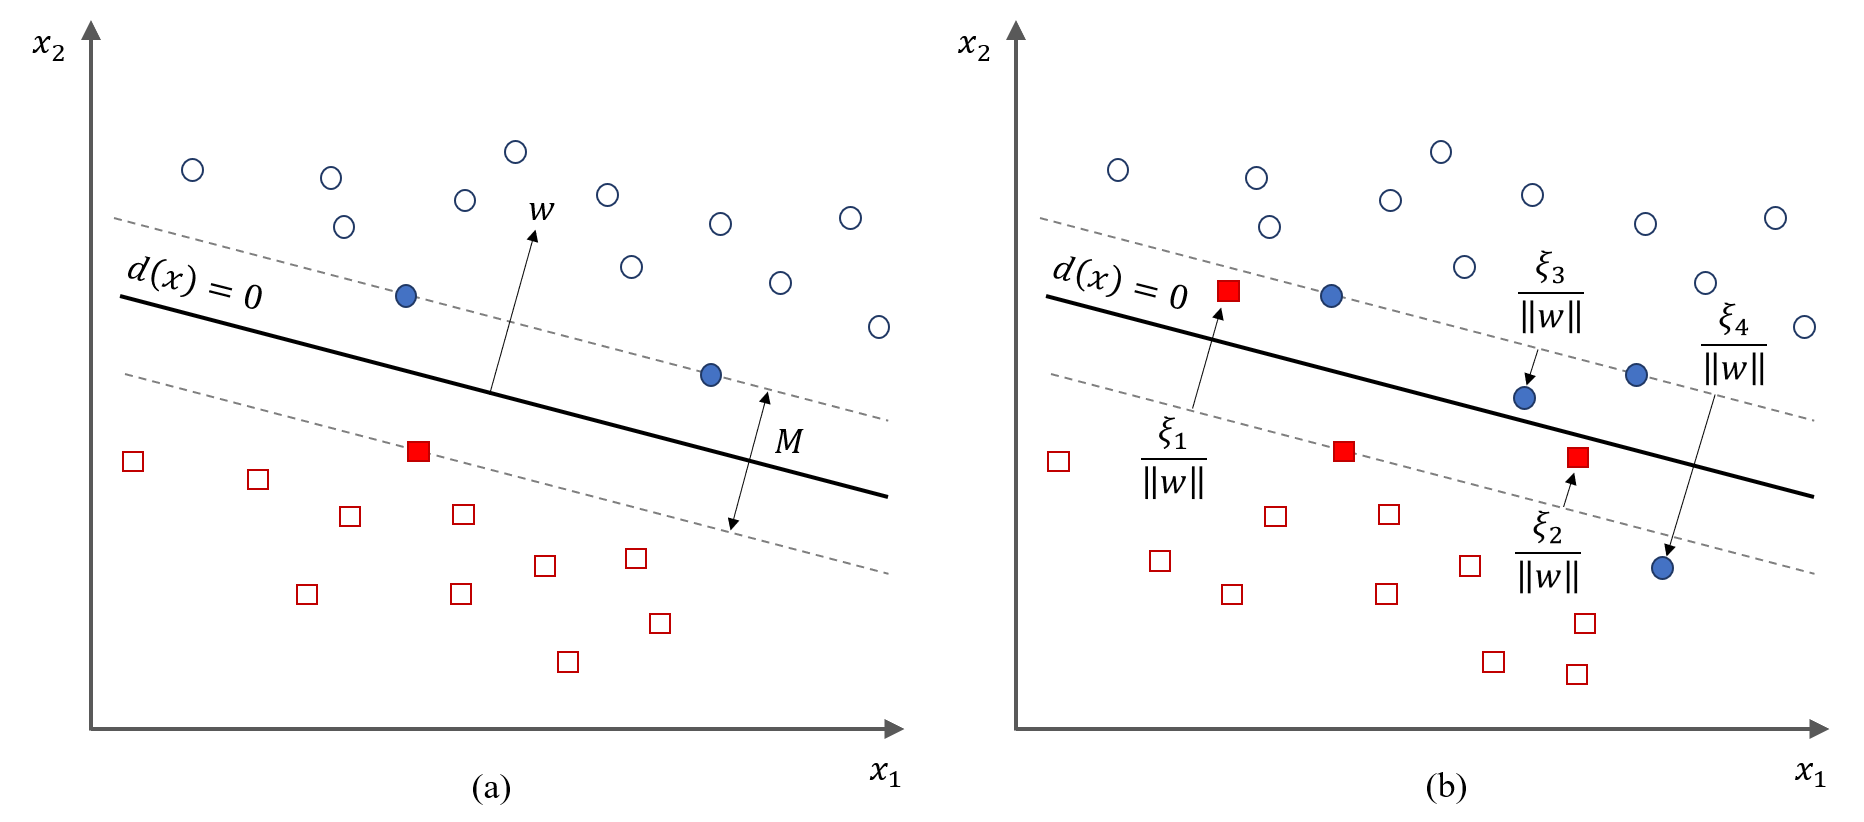
\includegraphics[width=1.0\textwidth]{resources/images/030-theoretical_framework/Framework_machine_learning_SVM.png}
        \smallcaption{Source: Author}
        \label{fig:frmwk_machine_learning_svm}
\end{figure}

In essence, the classification of data points into classes $(y = +1)$ or $(y = -1)$ in a multidimensional space can be accomplished by determining their position in relation to a hyperplane. Specifically, data points located on one side of the hyperplane $(d > 0)$ are associated with one class, whereas those on the other side $(d < 0)$ are attributed to the other class. The weight vector $w$, perpendicular to the hyperplane, determines the orientation of the hyperplane in the multidimensional space $\mathbb{R}^N$, while the bias $w_0$ shifts its position from the origin $\frac{w_0}{\parallel w \parallel}$. To maximize the margin $M$, the constraints are defined given all training examples {$x^{(i)}, y^{(i)}$}.

In practice, it is enough to retain the support vectors $x(i)$ with non-zero weights $\alpha_i$, as illustrated in Figure \ref{fig:frmwk_machine_learning_svm} by the filled circles and squares. Considering the linearity of the decision boundary, standard \gls{svm}s can only classify linearly separable data, however, \gls{svm}s have the ability to embed the data into a higher-dimensional space by applying a non-linear function $\Phi: \mathbb{R}^{N_1} \rightarrow \mathbb{R}^{N_2}$ to the input $x$, converting it to a non-linear space $\mathbb{R}^{N_2} (N_2 > N_1)$, where non-linearly spaced data can be separated using a linear decision function. Figure \ref{fig:frmwk_machine_learning_svm_kernel_trick} depicts this concept, where (a) is a two-dimensional training set with positive examples as black circles and negative examples as white circles. The true decision boundary is defined by the circumference, and (b) is the same data after mapping into a three-dimensional input space. The circular decision boundary in (a) becomes a linear decision boundary in three dimensions.

\begin{figure}[htbp]
    \raggedright
        \caption{Applying a non-linear transformation $\Phi$ to the input feature space to separate non-linearly spaced data with a linear hyperplane}
        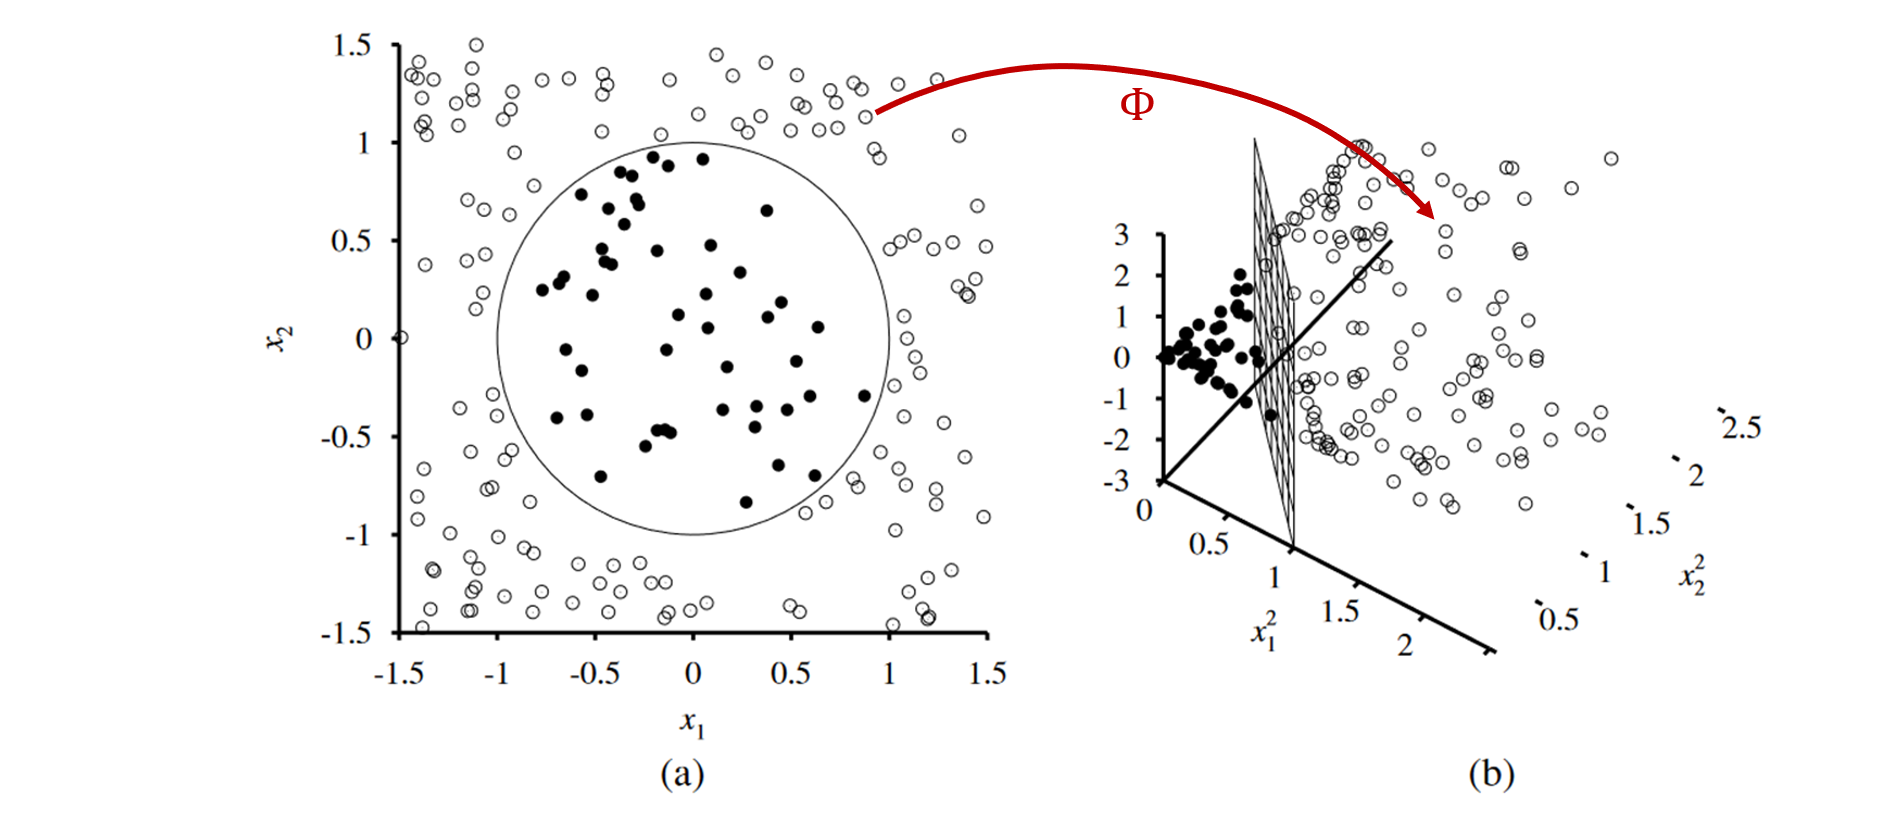
\includegraphics[width=1\textwidth]{resources/images/030-theoretical_framework/Framework_machine_learning_SVM_kernel_trick.png}
        \smallcaption{Source: Author "adapted from" \textcite{Russel2010}, page 747}
        \label{fig:frmwk_machine_learning_svm_kernel_trick}
\end{figure}

At this point, \textcite{Russel2010} highlight that the transformation $\Phi(x)$ to the input data presents significant computational challenges, and in some cases, it may be impracticable (e.g., with infinite $N_2$). However, the so-called \textbf{kernel trick} offers a solution by simplifying the transformation to a higher-order feature space through kernel evaluations. 

There are several kernel functions to be plugged into the \gls{svm}s, namely linear, polynomial, quadratic, and perceptron. Still, according to \textcite{Goodfellow2016}, the most commonly utilized kernel is the Gaussian kernel, also known as the \textbf{\gls{rbf} kernel}.

When dealing with inherently noisy data, a linear separator in a high-dimensional space might not be desirable. Instead, one seeks a decision surface in a lower-dimensional space that acknowledges the lack of clean separation between classes, reflecting the noisy nature of the data. This is achievable with the \textbf{soft margin} classifier, permitting examples to be situated on the incorrect side of the decision boundary while imposing a penalty proportional to the distance needed to relocate them to the correct side \cite{Russel2010}.

According to \textcite{Rothmund2018}, the penalty parameter $C$ essentially regulates the number of support vectors situated within the margin or on the 'wrong' side of the decision function ($\xi_i \neq 0$). When $C$ is small, the decision boundary becomes smoother, reducing the risk of overfitting. Conversely, a larger penalty $C$ results in a more intricate decision boundary that closely represents the training data. The objective is to determine a suitable parameter $C$ that captures the underlying trend in the training data without being excessively complex (leading to overfitting) or overly simplistic (resulting in underfitting). An example of soft margin $\frac{\xi_i}{\parallel w \parallel}$ is depicted in Figure \ref{fig:frmwk_machine_learning_svm} (b) by the filled circles and squares within the margin or even on the wrong side of the decision boundary.

\gls{svm} can be used for \textbf{multi-class discrimination} by combining several \gls{svm}s, thus creating a multi-class classifier for $N_c > 2$. Two methods are frequently available in the literature: the One-vs-Rest and the One-vs-One.

In the \textbf{One-vs-Rest} or \textbf{One-vs-All}, each class $c$ is trained individually, where samples belonging to class $c$ are labeled as positive $(y = 1)$, while the remaining samples are labeled as negative $(y = -1)$. The output class is determined by the maximum output score, such as the distance from the decision boundary.

The \textbf{One-vs-One} approach is more computationally demanding. In this method, $\frac{N_c(N_c-1)}{2}$ binary classifiers are trained, where each classifier corresponds to a unique pair of classes \{$c_i, c_j$\}. The binary output predictions from these classifiers are then aggregated by tallying the number of positive predictions for each class.

Although \gls{svm}s are highly sophisticated, they are not flawless: kernel machines encounter a significant computational burden during training, particularly with large datasets, and generic kernels often struggle to generalize well. According to \textcite{Goodfellow2016}, the modern incarnation of deep learning was designed to overcome these limitations of kernel machines, and its very renaissance began when \textcite{Hinton2006} demonstrated that a neural network could outperform the \gls{rbf} kernel \gls{svm} on the MNIST benchmark.


\subsubsection{Naïve Bayes}
\label{subsubsec:machine_learning_GNB}

The naïve Bayes classifier is a supervised machine learning algorithm that uses the principles of probability and Bayes' theorem to perform classification tasks. It is called naïve because it makes two simplifying assumptions: that the features are conditionally independent given the class and that all features have equal importance. Despite these unrealistic assumptions, the naïve Bayes classifier often works well in practice and is widely used for text classification, spam filtering, sentiment analysis, and more \cite{Barber2012}.

Depending on the choice of distribution, the naïve Bayes classifier can have different variants, such as the Bernoulli naïve Bayes can be used for binary features, the multinomial naïve Bayes can be used for categorical features, and the Gaussian naïve Bayes can be used for continuous features \cite{Friedman1997}. This study implemented the \textbf{\glsdisp{gnb}{Gaussian Naïve Bayes} (\gls{gnb})} algorithm from the Python library scikit-learn.

The naïve Bayes classifier has several advantages and disadvantages. Some of the advantages are that it is easy to implement, fast to train and test, robust to noise and irrelevant features, and scalable to large datasets. Some of the disadvantages are that it can suffer from zero-frequency problems, where a feature value that does not occur in the training data leads to a zero-posterior probability, and that it can perform poorly when the independence and equal importance assumptions are violated. To overcome these limitations, various smoothing techniques and feature selection methods can be applied \cite{Wickramasinghe2021}.

As a remark, \gls{glm} is a probabilistic model that assumes all the data points are generated from a mixture of several Gaussian distributions with unknown parameters. At the same time,  \gls{gmm} is a framework for modeling relationships between a response variable and one or more explanatory variables, which includes linear regression, logistic regression, Poisson regression, etc. While they all involve probability and modeling, including \gls{gnb}, they differ in their underlying assumptions, methodologies, and applications.


\subsubsection{Logistic Regression}
\label{subsubsec:machine_learning_logistic_regrassion}

\textbf{\glsdisp{lr}{Logistic Regression} (\gls{lr})} is a statistical method used for binary classification tasks, where the goal is to predict the probability that an instance belongs to one of two classes. Despite its name, logistic regression is a classification algorithm rather than a regression one.

The literature on \gls{lr} model is extensive, as evidenced by works such as \cite{Mitchell1997}, \cite{Bouguila2020}, and \cite{Russel2010}, therefore it suffices to state the basic idea, where the model applies the logistic function (also known as the sigmoid function) to the linear combination of input features. This function maps any real-valued number to the range between 0 and 1, which makes it suitable for representing probabilities.

\gls{lr} is trained using optimization algorithms, namely (some of them) maximum likelihood estimation, gradient descent, and limited-memory BFGS, or an online algorithm, such as stochastic gradient descent. The training aims to find the optimal values for the coefficients that minimize a cost function, typically the log loss or cross-entropy loss, which measures the difference between the predicted probabilities and the actual class labels in the training data.

\gls{lr} is inherently a binary classification algorithm, however, it can be extended to handle multiclass classification tasks through several strategies, namely:

\begin{itemize}
    \item \textbf{One-vs-Rest} or \textbf{One-vs-All}: by training one classifier per class and treating that class as the positive class and all other classes as the negative class. During prediction, the class with the highest probability from the individual classifiers is the winner;
    \item \textbf{Multinomial (Softmax)}: it handles multiple classes directly without needing multiple binary classifiers. Instead of predicting a binary outcome, it predicts the probabilities of each class using the softmax function, which normalizes the output into a probability distribution over multiple classes. During training, it minimizes the cross-entropy loss, which measures the difference between the predicted probabilities and the actual class labels;
    \item \textbf{Multiclass Hinge Loss}: this function penalizes predictions that are not sufficiently correct, aiming to maximize the margin between classes. This approach from \gls{svm} is often used when the emphasis is on maximizing margins between classes rather than directly optimizing probabilities.
\end{itemize}

This algorithm offers simplicity and interpretability, and furthermore, it has computational efficiency and resistance to overfitting, especially with smaller datasets. However, logistic regression assumes a linear relationship between features and outcomes, limiting its ability to capture complex patterns in the data. It struggles with non-linear relationships, large feature spaces, and outliers, which can affect its performance adversely \cite{Russel2010}.


\subsubsection{Random Forest (RF)}
\label{subsubsec:machine_learning_random_forest}

\textbf{\glsdisp{rf}{Random Forest} (\gls{rf})} is a popular ensemble learning method in machine learning. It's essentially a collection of decision trees, where each tree is trained on a different subset of the training data, and the final prediction is made by averaging (for regression) or voting (for classification) the predictions of all the individual trees. The method has essentially the following steps below according to \textcite{Breiman2001}, \textcite{Hartshorn2016}, and \textcite{Genuer2020}:

\textbf{Bootstrap sampling}: \gls{rf} builds multiple decision trees based on random subsets of the training data. This sampling technique, known as bootstrap sampling, involves selecting $k$ random samples with replacements from the original dataset, notably, some instances may appear multiple times in a subset, while others may not appear at all. Theoretically, $k$ samples will cover 2/3 of the original dataset, while the rest is called Out-Of-Bag.

\textbf{Feature randomness and decision tree construction}: When building each decision tree, \gls{rf} also introduces randomness in the features that can be considered at each split. Instead of considering all features at every split, it randomly selects a subset of $m$ features from $M$ total features and chooses the best split from that subset. This helps to decorrelate the trees, making them more diverse and less likely to overfit the training data. It is recommended to start with $m = \sqrt{M}$ number of selected features and then reduce or increase $m$ value until the minimum error for the Out-Of-Bag dataset is achieved. The best split is determined by assessing its quality using metrics from the "information theory", such as Gini impurity or entropy.

\textbf{Voting} or averaging for predictions: Once all the trees are constructed, predictions are made for new instances by each individual tree. For regression tasks, the final prediction is usually the average of the predictions of all trees, whereas, for classification tasks, the final prediction is determined by majority voting among all trees.

According to \textcite{Genuer2020}, \gls{rf} is among the preferred methods in the toolbox of statisticians and other data scientists due to its high accuracy, robustness to noise and irrelevant features, and ability to handle large datasets. It is also relatively easy to use and requires minimal parameter tuning, however, it can be computationally expensive and may not perform well on imbalanced datasets.


\subsubsection{Voting classifier}
\label{subsubsec:machine_learning_voting_classifer}

Voting classifier, also known as a probabilistic voting classifier, is an ensemble learning method in machine learning that combines multiple base classifiers and predicts the class label based on the probabilities of each class output by the individual classifiers.

Each base classifier in the ensemble independently predicts the class label for a given input. Instead of directly taking a majority vote, the voting classifier calculates the probabilities assigned to each class label by each base classifier, then it averages these probabilities for each class across all the base classifiers, and finally, the class label with the highest average probability is chosen as the final prediction \cite{Sarkar2019}.

This approach is particularly effective when the base classifiers are capable of providing probability estimates for their predictions, such as in the case of many classification algorithms like \gls{lr}, \gls{svm}s with probability outputs, or decision trees with probability outputs.

There are two types of voting classifiers: hard voting and soft voting. In hard voting, the final prediction is the class that receives the most votes from the individual models. In soft voting, the final prediction is the class with the highest average probability across all the individual models. Soft voting typically outperforms hard voting (where the majority vote is taken directly) because it considers the confidence levels of individual classifiers, resulting in more nuanced and often more accurate predictions.

According to \textcite{Sarkar2019}, this ensemble technique is robust against overfitting and outliers, as it averages out individual errors and biases. However, voting classifiers can be computationally intensive, especially when using a large number of diverse base classifiers. Additionally, interpretability may be compromised compared to single-model approaches like \gls{lr}, as the decision-making process involves multiple models. Nonetheless, voting classifiers are highly flexible and effective in a wide range of classification tasks, particularly when the individual base classifiers complement each other's strengths and weaknesses.


\subsection{Conclusion}
\label{subsec:machine_learning_conclusion}

The comprehensive analysis of the machine learning classifiers described in this section highlighted their key strengths and weaknesses with common themes, including considerations such as computational efficiency, generalization capability, robustness to noise, scalability to large datasets, and ease of implementation.  Additionally, the trade-offs between model complexity and interpretability are evident across different classifiers. While some of them excel in specific aspects like adaptability to new data \gls{k-nn}, others prioritize accuracy and robustness (\gls{rf}). Moreover, challenges such as overfitting, computational burden, and assumption violations are recurrent issues that must be addressed when selecting an appropriate classifier for \gls{esr} tasks. 


\section{NEURAL NETWORKS}
\label{sec:frmwk_neural_networks}

 Neural network, as initially proposed by psychologist Frank Rosenblatt, can be defined as a computational model inspired by the structure and function of the human brain, composed of interconnected artificial neurons, organized in layers, each responsible for performing specific computational tasks. These networks are capable of approximating complex non-linear relationships between inputs and outputs through a process called training, where the network adjusts its internal weights based on a given set of example data. This adaptive learning enables neural networks to recognize patterns, make predictions, and solve various types of problems \cite{Rosenblatt1958}.
 

\subsection{Artificial Neural Network (ANN)}
\label{subsec:neural_network_ANN}

The cornerstone of \gls{ann} lies in a fundamental mathematical model of an artificial neuron introduced by McCulloch-Pitts in 1943. This model serves as the groundwork for computational methodologies in the realm of learning, describing the properties of a single neuron by forming a linear combination of the outputs of other neurons, which is then transformed using a nonlinear function \cite{Bishop2023}. An artificial neuron aggregates the input values {$x_1, x_2, \ldots , x_M$} through a linear combination process illustrated by Figure \ref{fig:frmwk_ann_artificial_neuron} (a). Each input $x_i$ is assigned a weight $w_i$, which is used to scale or weight the input value. The total of the weighted inputs, along with the bias $b$, is defined as the activation $a$, and after it passes through a non-linear activation function $\sigma(a)$, it produces the output state $y_j$ of the neuron. 

\begin{equation}
    \label{eq:ann_activation}
    a = \sum_{i=1}^M w_i \cdot x_i + b \quad\quad y_j = \sigma(a)
\end{equation}

This linear combination can be expressed by the dot product of a weighted vector $W$ and the input vector $X$, given by:

\begin{equation}
    \label{eq:ann_activation_outpu}
    y_j = \sigma  \left( W^TX +b \right)
\end{equation}

The trainable weight vector $w$ plays a crucial role in determining the significance of an input to a neuron's output. Similarly, the trainable bias $b$ sets the operational point within the non-linear activation function $\sigma(a)$. The activation function $\sigma(a)$ mimics its biological counterpart by limiting the strength of electrical spikes traveling through the axon to a specific range, as illustrated in Figure \ref{fig:frmwk_ann_artificial_neuron} (b).

According to \textcite{Bishop2023}, frequently utilized general-purpose non-linear activation functions to constrain the neuron's state $y$ within a reasonable range include hyperbolic tangent (Tanh) and \gls{relu}. Sigmoid and softmax are commonly employed at the neural network's output layer for classification tasks, transforming the input into a probability-like range between 0 and 1 as shown in Figure \ref{fig:frmwk_ann_activation_functions} (a) to (d). Specifically, sigmoid is suitable for binary classification, while softmax performs better for multi-class classification scenarios. In both cases, they are preferred for their regularization benefits and faster training compared to hyperbolic tangent activations. A decision function is typically implemented to obtain a discrete class from these continuous probability outputs. In single-label multi-class classification, the argmax function is commonly used to select the class with the highest probability value. 

\begin{figure}[htbp]
    \raggedright
        \caption{Artificial neuron mimicking a biological neuron}
        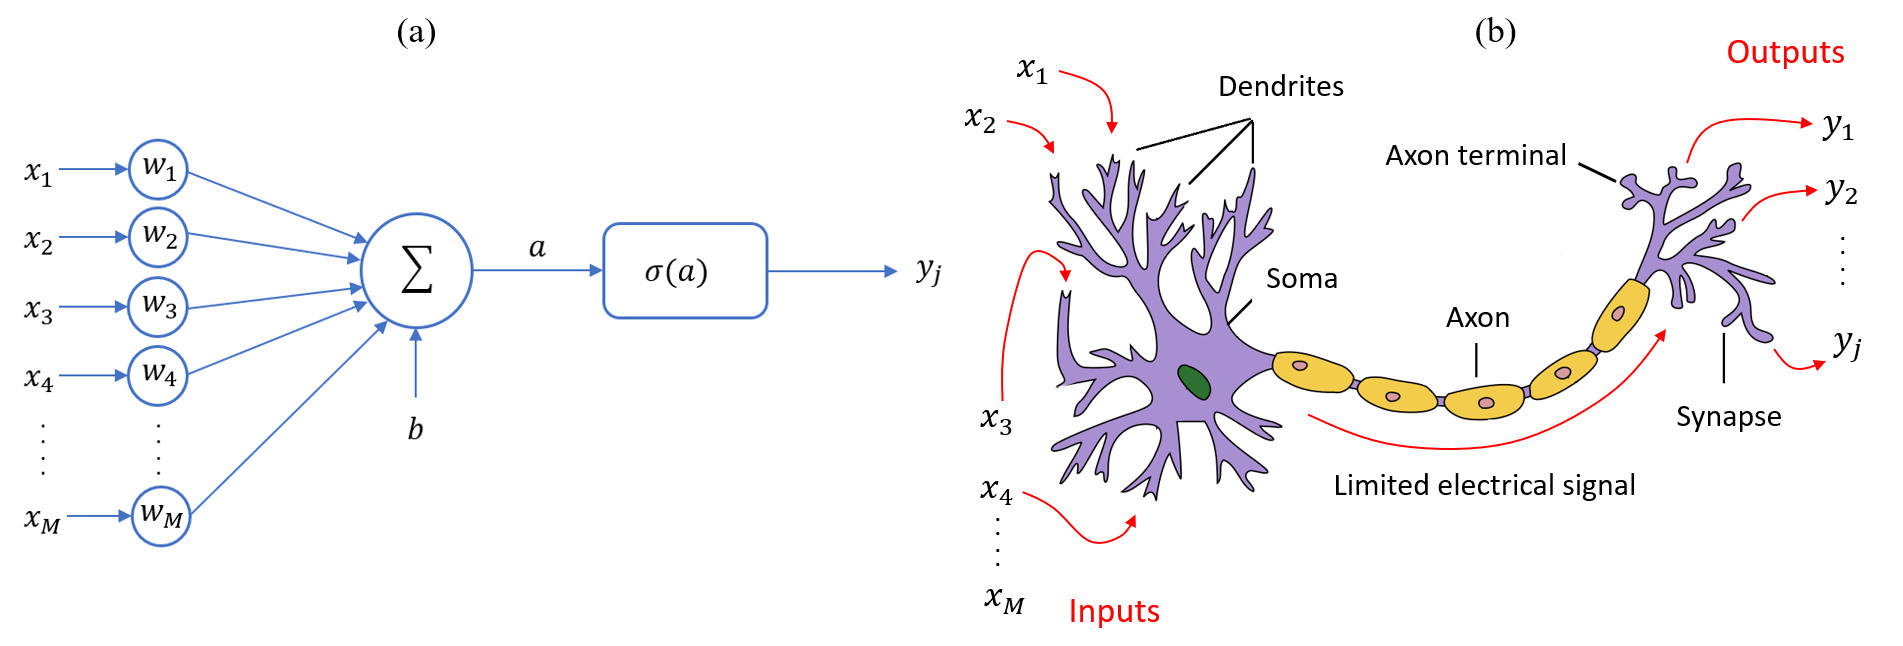
\includegraphics[width=1\textwidth]{resources/images/030-theoretical_framework/Framework_ann_neuron.png}
        \smallcaption{Source: Author}
        \label{fig:frmwk_ann_artificial_neuron}
\end{figure}

\begin{figure}[htbp]
    \raggedright
        \caption{Common activation functions}
        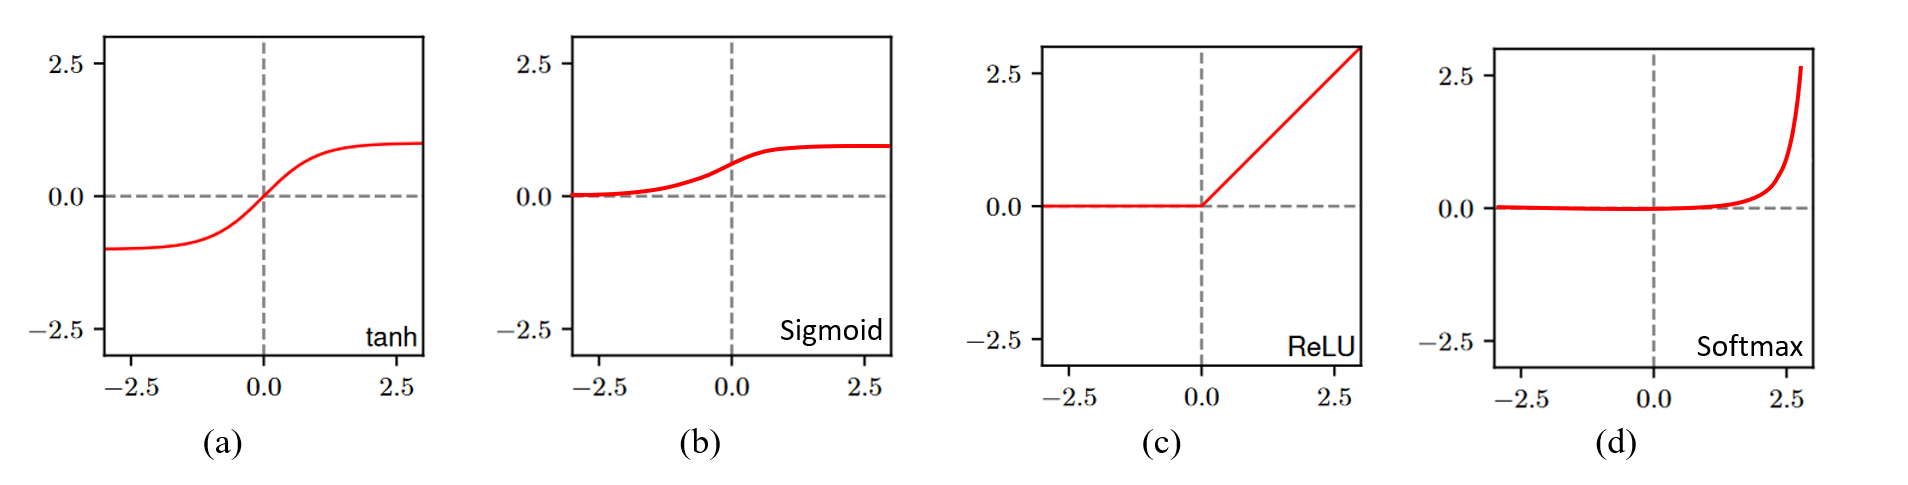
\includegraphics[width=1\textwidth]{resources/images/030-theoretical_framework/Framework_ann_activation_function.png}
        \smallcaption{Source: Author "adapted from" \textcite{Bishop2023}, page 184}
        \label{fig:frmwk_ann_activation_functions}
\end{figure}

One of the most popular \gls{ann} is the \textbf{\gls{mlp}}, a feedforward neural network model that consists of multiple layers of nodes (neurons), each layer fully connected to the next layer, organized consecutively as input, hidden and output layer as depicted in Figure \ref{fig:frmwk_ann_mlp}. The \gls{mlp} is characterized by its ability to learn nonlinear models by using an activation function that introduces non-linearity into the network's decision-making process \cite{Mitchell1997}.

According to \textcite{Russel2010}, the first layer, or the input layer, receives input data features where each node represents a feature of the input data. Followed by hidden layers $L$, which are the intermediate layers between the input and output layers where each node in a hidden layer $l$ consisting of $m^{(l)}$ parallel nodes receives input from all the nodes in the previous layer and applies an activation function $\sigma^{(l)}(a_i^{(l)})$ to the weighted sum of those inputs and fed to the inputs of the next layer ($l+1$). The last layer, or output layer ($L+1$), produces the network output vector. The number of nodes in this layer depends on the problem type, for instance, for binary classification, one might have one output node representing the probability of belonging to one class, and its complement representing the probability of belonging to the other class. 

\gls{mlp}s are trained using supervised learning methods like backpropagation, where the network adjusts its internal parameters (weights and biases) iteratively to minimize the difference between its output and the desired output for a given set of input data. The training process undergoes by optimizing a specified objective function, also known as a loss function. In the context of supervised learning, the predominant technique utilized is mini-batch \textbf{\gls{sgd}} coupled with \textbf{Backpropagation}, particularly for classification tasks. The cross-entropy function, commonly referred to as log-loss, is frequently employed. The log-loss function exhibits a tendency towards infinity as the predicted probability of the true class approaches zero, imposing significant penalties for wrong predictions. \textbf{Categorical cross-entropy} serves as an extension of binary cross-entropy tailored for scenarios involving multi-class, and according to the problem and the classification tasks, the literature provides additional loss functions, such as Logistic Loss, Mean Squared Error, and Mean Absolute Error. The process of generating predictions through a feedforward neural network and subsequently evaluating the loss function facilitates the assessment of the model's performance, and to enhance it, an optimization algorithm is applied to determine necessary adjustments to the model parameters. There are several options for the optimization algorithm, such as \gls{sgd}, Adam, RMSprop, etc. Still, they all generate a gradient of a function that quantifies the rate and direction of its output variations in response to incremental modifications in its inputs, computed through partial derivatives of the function \cite{Bishop2023}. 

\begin{figure}[htbp]
    \raggedright
        \caption{MLP with $M$ inputs, $L$ hidden layers, each with $m^{(l)}$ nodes and $N_c = 3$ output nodes. Arrows represent weighted connections between nodes}
        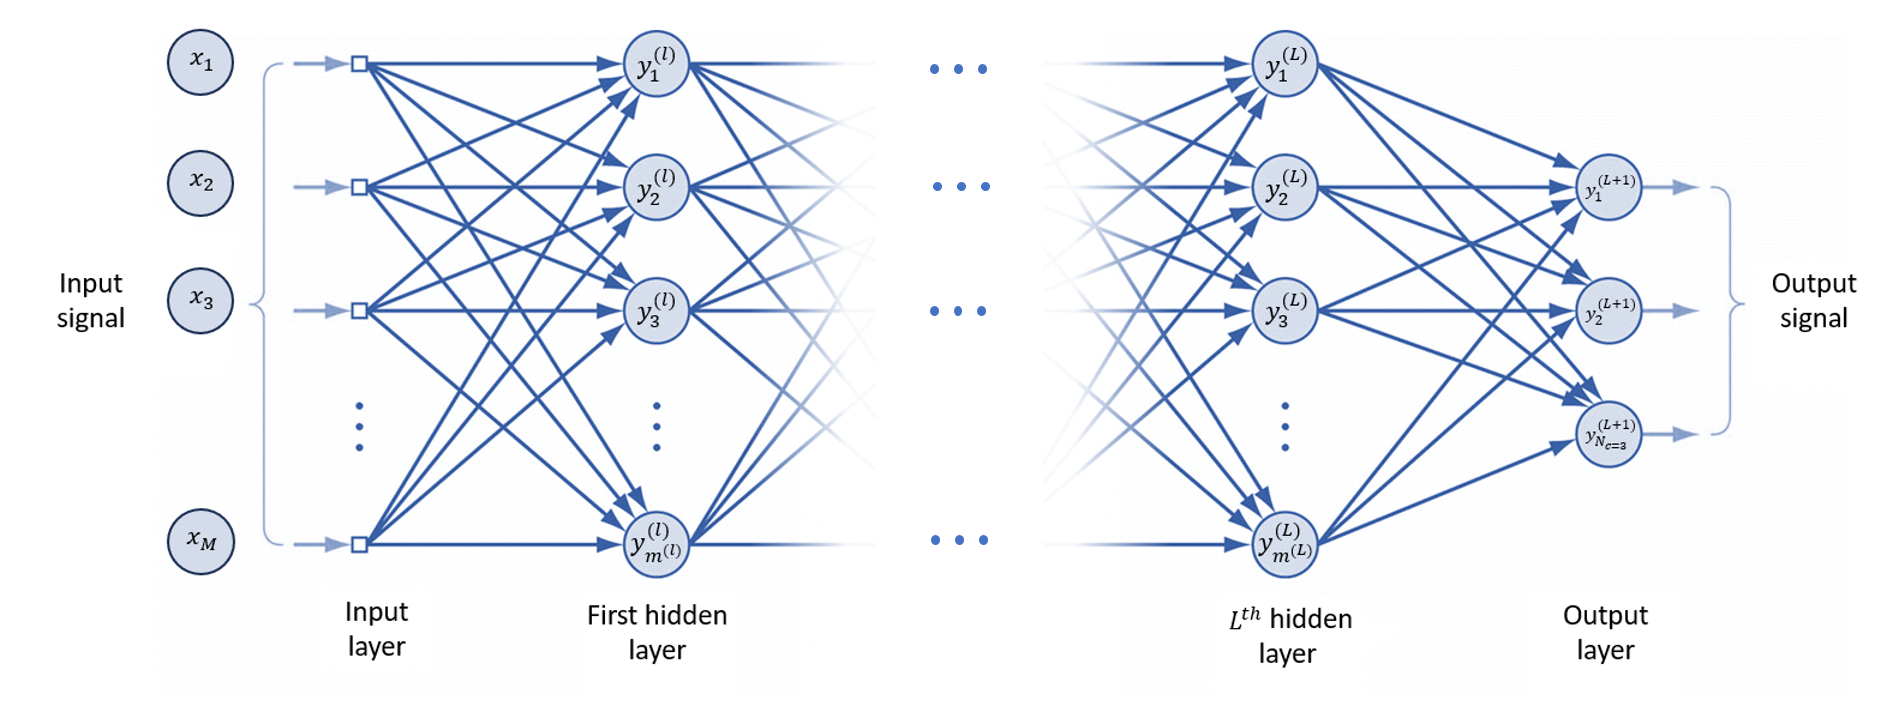
\includegraphics[width=1\textwidth]{resources/images/030-theoretical_framework/Framework_ann_mlp.png}
        \smallcaption{Source: Author}
        \label{fig:frmwk_ann_mlp}
\end{figure}

The fundamental mechanism for computing gradients in a \gls{mlp} is through the utilization of backpropagation \cite{Rumelhart1986}, which involves iteratively propagating the error signals from the output layer back to the input layer by calculating the partial derivatives with respect to the inputs from the preceding layer. This process enables the determination of gradients for each weight and each bias in the network, and subsequently, once the gradients are obtained, weight adjustments are made by moving in the opposite direction of the gradient. To control the magnitude of this adjustment, each step of this process is scaled by a \index{hyperparameter}hyperparameter known as the \textbf{learning rate}, which typically falls within the range of $10^{-7}$ to $10^{-2}$. Selecting an appropriate learning rate is crucial, as excessively small values may lead to convergence issues or local minima, whereas excessively large values can hinder training convergence. There are no shortcuts in this process, and the "rule of thumb" for defining the learning rate is to assess the model results using cross-validation, a systematic and rigorous technique for evaluating the performance of a learning model and for selecting the best hyperparameters.

Optimization algorithms that utilize the complete training set for updating each parameter are referred to as batch training or deterministic gradient methods, where the batch size is equivalent to the total number of observations in the training set. In \textbf{mini-batch} Gradient Descent, the training set is divided into fixed-size batches, and the loss function and model parameter updates are calculated for each batch, allowing for processing large datasets without the need to store all the training data in memory simultaneously. The batch size, a hyperparameter, must be chosen carefully to ensure that the batch loss provides a reasonable approximation of the overall training set loss while still fitting into memory \cite{Bishop2023}. Each complete iteration through the entire training dataset is referred to as an \textbf{epoch}, with multiple epochs typically being conducted during training. 

While Gradient Descent does not ensure the discovery of a globally optimal minimum, appropriate hyperparameter selections typically lead to satisfactory local minima. According to \textcite{Choromanska2015}, achieving a global optimum on the training set may not be advantageous, as it is unlikely to result in a strong generalized model.


\subsection{Convolutional Neural Network (CNN)}
\label{subsec:convolutional_neural_network_CNN}

\gls{cnn}, as introduced by \textcite{Lecun1998}, is a specialized type of neural network designed for processing data with a structured, grid-like topology, and it has demonstrated significant success in real-world applications. This can include various forms of data, such as time-series data represented as a 1D grid with samples taken at regular intervals and image data represented as a 2D grid of pixels. The term "convolutional neural network" reflects the utilization of the mathematical process known as convolution, a specialized form of linear operation within the network architecture. \textcite{Goodfellow2016} defined a convolutional network as a simple neural network that uses convolution instead of general matrix multiplication in at least one of its layers.

Essentially, \gls{cnn}s are complex architectures comprised of multiple convolutional layers, followed by pooling/down-sampling layers and fully-connected layers of artificial neurons. The primary function of convolutional layers is to correlate segments of input data with pre-trained filter kernels to identify patterns, resulting in a high output score for matching features. By incorporating additional convolutional layers, increasingly intricate patterns can be extracted from the input data. Figure \ref{fig:frmwk_cnn_LeNet-5} illustrates the architecture of a \gls{cnn} with two convolutional layers, pooling layers, and fully-connected layers serving as a classifier as proposed by Lecun in the LeNet-5.

\begin{figure}[htbp]
    \raggedright
        \caption{Example of CNN (LeNet-5) proposed by LeCun}
        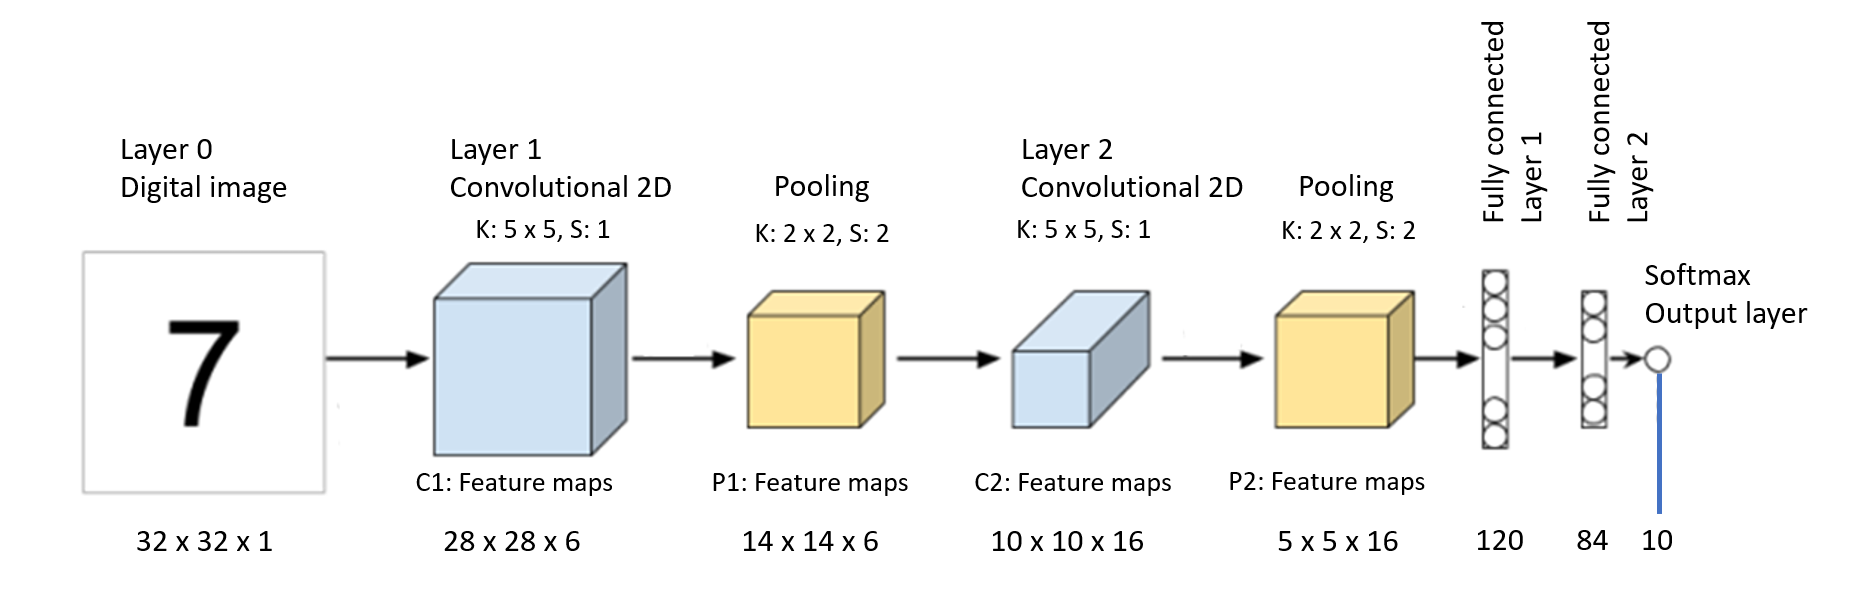
\includegraphics[width=1\textwidth]{resources/images/030-theoretical_framework/Framework_cnn_LeNet-5.png}
        \smallcaption{Source: Author "adapted from" \textcite{Lecun1998}, page 2283}
        \label{fig:frmwk_cnn_LeNet-5}
\end{figure}

According to \textcite{Goodfellow2016} and \textcite{Rothmund2018}, the convolution operation is typically denoted with an asterisk (*), and a discrete convolution for functions $x(t)$ and $k(t)$ is expressed as:

\begin{equation}
    \label{eq:cnn_discrete_convolution}
    s(t) = (x * k)(t) = \int x(\tau)k(t-\tau)d\tau
\end{equation}

Given that $x$ and $k$ are defined solely at discrete intervals, the discrete convolution, denoted as $s_i$, can be defined as:

\begin{equation}
    \label{eq:cnn_discrete_convolution_si}
    s_i = (x * k)_i = \sum_{n=-\infty}^{\infty} x_i \cdot k_{i-n} 
\end{equation}

Filter kernels may vary in dimensionality, being one-dimensional, two-dimensional, or three-dimensional, depending on the format of the input data. In the context of image recognition, the convolution process enables the representation of various beneficial transformations on two-dimensional data through the selection of different weights within the kernel. Examples include edge detection (horizontal, vertical, diagonal) and smoothing filters (mean, Gaussian). As the weights of the kernels in a convolutional layer are trained, they become adept at identifying local features specific to the training dataset. In cases involving multiple input channels, a single kernel is applied across all input channels, with the results at a given location and the bias being aggregated to generate the output \cite{Bishop2023}. 

Given a two-dimensional kernel $K$ with dimensions $h_1$ × $h_2$ and an input image $X$ with dimensions $m_1$ × $m_2$, the convolution operation can be expressed according to \textcite{Rothmund2018} as:

\begin{equation}
    \label{eq:cnn_convolution_2D_1}
    s_{i, j}=(X * K)_{i, j}=\sum_{m=1}^{h_1} \sum_{n=1}^{h_2} x_{i-m, j-n} \cdot k_{m, n}
\end{equation}

With input $X$ and the kernel $K$ yielding the two-dimensional output $S$.

\begin{equation}
    \label{eq:cnn_convolution_2D_2}
    K=\left[\begin{array}{llll}
    k_{0,0} & k_{0,1} & \cdots & k_{0, l_2} \\
    k_{1,0} & k_{1,1} & \cdots & k_{1, l_2} \\
    \vdots & \vdots & \ddots & \vdots \\
    k_{l_1, 0} & k_{l_1, 1} & \cdots & k_{l_1, l_2}
    \end{array}\right] \quad \text { and } \quad X=\left[\begin{array}{llll}
    x_{0,0} & x_{0,1} & \cdots & x_{0, m_2} \\
    x_{1,0} & x_{1,1} & \cdots & x_{1, m_2} \\
    \vdots & \vdots & \ddots & \vdots \\
    x_{m_1, 0} & x_{m_1, 1} & \cdots & x_{m_1, m_2}
    \end{array}\right]
\end{equation}

Figure \ref{fig:frmwk_cnn_convolution_example} illustrates the process of a discrete two-dimensional convolution using a small 2×2 kernel designed to detect vertical edges. The kernel is applied to a larger 5×5 dimension input image and computed according to equation \ref{eq:cnn_convolution_2D_1}. The resulting output image highlights the vertical edge with a darker color, while the horizontal edge appears less pronounced. It is important to note that zero-padding was not utilized in this example, leading to a reduction in dimensions for the output image $S$ (4×4). If zero-padding, also named \textit{same padding}, was applied, zeros would be added to the input image's borders in such a way that the output image $S$ would have the same spatial dimensions as the input image $X$.

\begin{figure}[htbp]
    \raggedright
        \caption{2D discrete convolution performed on input image $X$ with dimensions of 5×5 using a filter kernel $K$ with dimensions of 2×2, yielding an output image of size 4×4. The filter kernel is designed to detect and enhance vertical lines in the image.}
        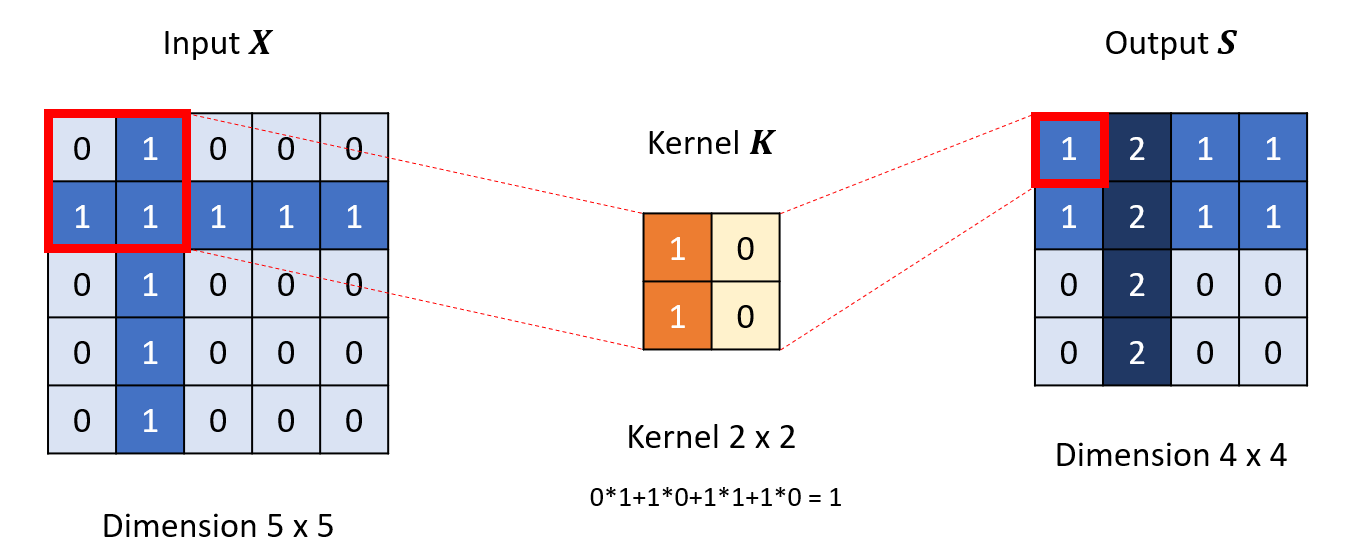
\includegraphics[width=.9\textwidth]{resources/images/030-theoretical_framework/Framework_cnn_example.png}
        \smallcaption{Source: Author}
        \label{fig:frmwk_cnn_convolution_example}
\end{figure}

The input of a two-dimensional \textbf{convolutional layer} $l$ consists of a three-dimensional array containing $n_1^{(l)}$ two-dimensional feature maps with dimensions $n_2^{(l)} \times n_3^{(l)}$. For spectrograms or black and white images, the number of channels or feature maps is denoted as $n_1^{(1)}=1$, while for a colored RGB image (the RGB color space is an additive color model, describing a color in three channels, representing the colors red, green and blue) the number of channels would be $n_1^{(1)}=3$. Each convolutional layer comprises $m_1 \cdot n_1$ filter kernels $K_{i,j}$, each with dimensions $h_1^{(l)} \times h_2^{(l)}$, resulting in $m_1^{(l)}$ two-dimensional feature maps with dimensions $m_1^{(l)} \times m_2^{(l)}$ at the output. These filter kernels, denoted as $K_{i,j}$, are responsible for identifying specific patterns across the input data $X_j$. 

The output feature maps $Y_i^{(l)}$ for layer $l$ are obtained by summing the discrete convolutions of the trainable filter kernels $K_{i,j}$ with the input feature maps $X_j$ and a trainable bias term $b_i^{(l)}$. With $i = 1, 2,\ldots, m_1, j = 1, 2,\ldots, n_1$ and $\sigma^{(l)}$ as the non-linear transformation function, it compute as:

\begin{equation}
    \label{eq:cnn_convolutional_layer}
    Y_i^{(l)}=\sigma^{(l)}\left(b_i^{(l)}+\sum_{j=1}^{n_1^{(l)}} K_{i, j}^{(l)} * X_j^{(l)}\right)
\end{equation}


Subsampling the data as it progresses through the convolutional layers is crucial for enhancing the model's ability to learn larger and more intricate features. This process is achieved through \textbf{pooling layers}, such as the 2D pooling operation with a $f_1$ x $f_2$ sized \textbf{filter} and a \textbf{stride} matching the operation size. Each channel is independently processed in the pooling operation, which outputs either the average value of the input in \textit{average pooling} or the maximum value in \textit{max pooling}, as depicted in Figure \ref{fig:frmwk_cnn_pooling}. In other words, pooling layers don't learn any pattern in the network; rather, they reduce the resolution of the output feature maps from preceding convolutional layers ($Y_i^{(l-1)}$) by applying an filter window of size $f_1$ x $f_2$ with a stride of $s_1$ x $s_2$.

\begin{figure}[htbp]
    \raggedright
        \caption{Pooling examples on a two-dimensional input image $X$ of size $m_1$ × $m_2$ = 4×4 with pool size $f_1$ × $f_2$ = 2×2 and stride $s_1$ × $s_2$ = $f_1$ × $f_2$ (no overlap).}
        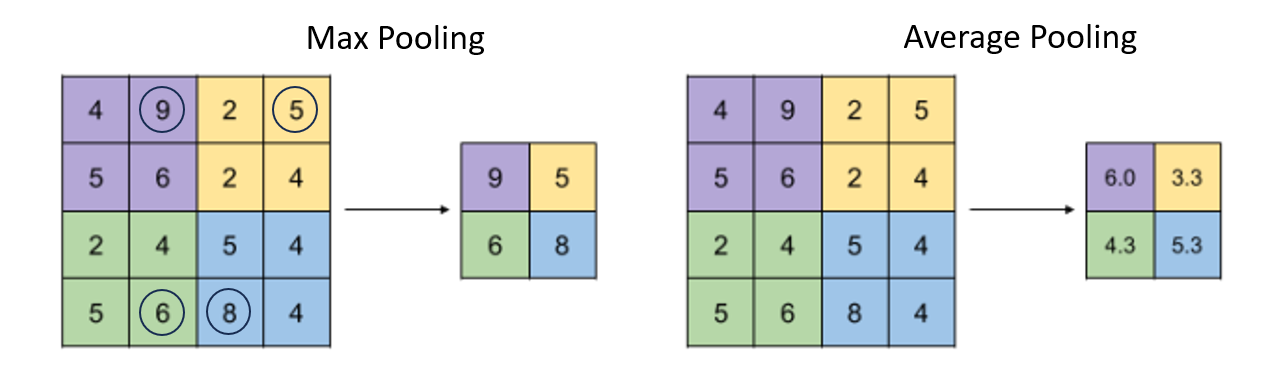
\includegraphics[width=.9\textwidth]{resources/images/030-theoretical_framework/Framework_cnn_pooling.png}
        \smallcaption{Source: Author "adapted from" \textcite{IndoML2018}}
        \label{fig:frmwk_cnn_pooling}
\end{figure}

As a remark, \gls{lstm} networks have recently emerged as a promising alternative to \gls{cnn}s in the field of environmental sound recognition. Unlike \gls{cnn}s, which are primarily designed for image processing tasks, \gls{lstm}s are well-suited for sequential data analysis due to their ability to capture long-range dependencies and temporal dynamics in audio signals \cite{Bubashait2021}. By modeling the temporal relationships within sound sequences, \gls{lstm}s can effectively learn intricate patterns and nuances in acoustic data, making them a valuable tool to be further investigated for tasks in the field of \gls{esr}.


\subsection{Conclusion}
\label{sec:frmwk_neural_networks_conclusion}

In the context of \gls{esr}, neural networks are able to offer distinct advantages. \gls{mlp}s provide a strong foundation for understanding basic sound patterns and relationships using the interconnection of hidden layers and neurons, while \gls{cnn} 1D excels in capturing temporal dependencies within sound data. On the other hand, \gls{cnn} 2D is particularly effective in extracting spatial features from spectrogram representations of environmental sounds. By leveraging the unique strengths of each model, a more robust and accurate \gls{esr} algorithm can be developed for autonomous vehicles.


\section{ELECTRONIC CONTROL UNIT}
\label{sec:frmwk_electronic_control_unit}

An \glsdisp{ecu}{Electronic Control Unit} (\gls{ecu}) is an embedded system found in automotive electronics that regulates one or more electrical systems or subsystems within a motor vehicle. To address the requirements of these systems and subsystems, a clear trend in the automotive sector involves the growing prevalence of electronic components within vehicles that are vital for controlling propulsion, chassis, body functions, in-vehicle networks, and driving information systems. Depending on the system, the \gls{ecu} receives a specific acronym, for example, engine control module (ECM), powertrain control module (PCM), transmission control module (TCM), brake control module (BCM or EBCM), central control module (CCM), body control module (BCM), etc. Although colloquially referred to as the car's computer, it is important to note that these \gls{ecu}s are distinct individual computers running \gls{soc} rather than a single unit \cite{Aptiv2020}.


\subsection{Vehicle EE architecture}
\label{subsec:ECU_common_units_in_market}

This section will present a brief overview of where the \gls{esr} algorithm could be deployed or embedded within the vehicle \gls{ee} architecture considering the findings of \textcite{Zhu2021}, and it will not dwell on the intricacies and details of the architecture itself but rather will focus on the application deployment considering a regular passenger car and an autonomous vehicle.

Assuming a \textbf{centralized gateway architecture} with the \gls{esr} algorithm embedded on a specific \gls{ecu} would have the advantage of improving functional safety given that the gateway converts different protocols and regulates network traffic, on the other hand,  the number of \gls{ecu}s have been increasing constantly, which lead to more complexity in the gateway and ultimately, it may be harmful for security. A more updated architecture, such a \textbf{domain-based}, would integrate portions of the \gls{ecu} containing specific software components thus reducing material cost and weight in manufacturing processes. Additionally, the overhead in the gateway and bottleneck of multiples \gls{ecu}s will be reduced, conversely, the potential downsize are delays that may be introduced between sensors and actuators. \textbf{Zone-based architecture} is currently a trend, and many automakers are developing their future products based on this concept. The main advantage is that the electronic components can be integrated based on their physical location in the vehicle, reducing cabling, especially for Ethernet, with the combination of communication and power. The disadvantage is that the architecture entails higher software platform requirements due to the location cluster.

Shifting to autonomous vehicles, it is "common sense" that Tesla is in the vanguard of hardware and software development, and according to \textcite{Lindholm2008}, the underlying structure of the Tesla architecture relies on a flexible processor array based on the GeForce 8800 \gls{gpu}, with 128 streaming-processor (SP) cores, organized into 16 streaming multiprocessors (SMs) that are further grouped into eight separate processing units referred to as texture/processor clusters (TPCs). Notably, this is just a small part of the so-called HW4 infotainment system hacked by \textcite{Teslanorth2023} on the Tesla Model. For obvious reasons, Tesla does not disclaim their infotainment technical specifications, and therefore, the information that the HW4 infotainment system has 128 \gls{g}\gls{b} of storage capacity and 8 \gls{g}\gls{b} of \gls{ram} is assumed to be valid.

The Tesla architecture, developed by NVIDIA, is considered to be the pioneering platform for ubiquitous supercomputing. Its success is attributed to its compatibility with C programming language and the CUDA software development environment, which allows for the efficient deployment of computationally intensive parallel-computing and graphics applications. As transistors become more densely packed in the future, this architecture will be able to effortlessly scale processor parallelism, memory partitions, and overall performance \cite{Lindholm2008}. Based on this conclusion, it is plausible to assume that \gls{esr} algorithms could be deployed in autonomous vehicles using only embedded software in the current \gls{ee} architecture. This approach would bring added value but not extra costs on hardware. It may be necessary to consider additional sensors like external microphone arrays, though.


\subsection{High-end general-purpose embedded platform}
\label{subsec:ECU_high-end-platform}

In the realm of computing, specialized architectures, and general-purpose platforms play distinct roles in catering to various computational needs. \glsdisp{fpga}{Field-Programmable Gate Arrays} (\gls{fpga}) and \glsdisp{tpu}{Tensor Processing Units} (\gls{tpu}) are examples of specialized architectures tailored for accelerating machine learning tasks, particularly those involving tensor operations. On the other hand, high-end general-purpose platforms like Raspberry Pi offer versatile computing capabilities at a more accessible price point. Considering the current platform utilized in the C-Bot, this study will focus on the high-end general-purpose platform Raspberry Pi 4, model B \cite{Raspberry2023}, however, this section will briefly explain the most common architectures for machine learning tasks, given that \gls{ecu}s for the automotive industry, especially the ones designed for autonomous vehicles, can have a \gls{fpga} or \gls{tpu} technology embedded in its hardware.

\textbf{\gls{fpga}} is a customizable integrated circuit that can be reconfigured after manufacturing, making it highly flexible for various applications, including accelerating specific algorithms and tasks. It is often used in specialized computing tasks, including machine learning acceleration, digital signal processing, and hardware emulation, because they offer parallelism and low-latency processing, making them suitable for real-time applications where performance is critical. Latest technologies in \gls{fpga} include Xilinx Versal AI Core series, advancements in high-level synthesis tools for easier programming, integration with high-speed interfaces like PCIe Gen4 for faster data transfer, and the incorporation of hardened IP blocks for common functions, such as memory controllers and DSP blocks \cite{IntelFPGA2024}.

\textbf{\gls{tpu}}s Google's custom-built ASIC (Application-Specific Integrated Circuit) is designed specifically for accelerating machine learning workloads, more specifically, optimized for \index{Tensorflow}TensorFlow \cite{TensorFl23}, Google's open-source machine learning framework, but can also be used with other frameworks like PyTorch and JAX. They excel at both training and inference tasks and are known for their high performance and energy efficiency. Recent advancements in \gls{tpu} technology include the development of second and third-generation \gls{tpu}s, which feature higher computational capabilities, increased memory bandwidth, and improved support for mixed-precision computing (Coral Dev Board). Additionally, there is ongoing research into integrating \gls{tpu}s with Google's Cloud AI infrastructure to provide scalable and efficient machine learning solutions for various industries \cite{GoogleTPU2024}.

\textbf{Raspberry Pi} is a series of small single-board computers developed by the Raspberry Pi Foundation, and although not as powerful or specialized as \gls{fpga} or \gls{tpu}, Raspberry Pi offers a cost-effective solution for various computing tasks, from basic programming to IoT (Internet of Things) projects. The latest Raspberry Pi models feature significant improvements in processing power, memory, and connectivity options compared to earlier versions; for example, Raspberry Pi 5 introduced a quad-core ARM Cortex-A72 processor, up to 8\gls{g}\gls{b} of RAM, USB 3.0 ports, Gigabit Ethernet, and support for dual 4K displays.
Recent developments in the Raspberry Pi ecosystem include the release of Raspberry Pi OS, a Debian-based operating system optimized for Raspberry Pi hardware, and the expansion of software and hardware peripherals compatible with the platform \cite{Raspberry2023}.


\subsection{Conclusion}
\label{subsec:ECU_conclusion}

Upon initial examination, it appears more reasonable, regardless of whether using a domain-based or zone-based architecture, to leverage the capabilities of current sophisticated electronic systems available in regular passenger vehicles, like infotainment devices or head units, in order to integrate the \gls{esr} algorithm. These systems are already equipped with ample storage and computational power to effectively execute the algorithms, moreover, they often possess advanced embedded audio processing algorithms and beam-forming features, further enhancing their suitability for this purpose. On the other hand, high-end general-purpose platforms like Raspberry Pi offer versatile computing capabilities at a more accessible price point, especially for proof-of-concepts or advanced prototypes like the C-Bot.

